\documentclass[11pt,a4paper]{report}
\linespread{1.25}

% dissertation.tex
% 
%
% MSc Project report / Thesis
% Author: Oliver Earl <ole4@aber.ac.uk>
% 
% This LaTeX template was constructed by Dr. Hannah Dee (hmd1@aber.ac.uk)
% and Neil Taylor (nst@aber.ac.uk) based on the Leeds thesis template and the
% Group Project template for Computer Science in Aberystwyth University.
% I credit it accordingly.
%
% Comments and suggestions of the template itself should be directed to its
% GitHub repository: https://github.com/digidol/MMP
%
% The template is designed to be used with pdflatex and may require modification
% to run with a different LaTeX engine. 
%
% I am using LaTeX Workshop for Visual Studio Code for authoring, which compiles
% my mark-up automatically. You can also build manually by running the included 
% build.sh file. Alternatively:
%
% pdflatex dissertation
% bibtex dissertation
% pdflatex dissertaton (run this twice)
%
% Either will result in dissertation.pdf being compiled.
%
% I personally use the aforementioned extension for vscode to perform word
% counts, but I've included the TeXcount Perl 5 script in the repository to 
% do this if desired. If you run build.sh, it will run this script for you
% after compilation.
%
% Naturally, I didn't write it, so you can find it here:
% https://app.uio.no/ifi/texcount/

\usepackage{mmp}
\usepackage{cite}
\usepackage{pdfpages}
\usepackage{nameref}
\usepackage{listings}

\begin{document}

%TC:ignore

% all of the include directives below refer to tex files
% so %TC:ignore 

\title{Web-Based Rostering System for Volunteer Worked Organisations}
\author{Oliver Earl}
\authoremail{ole4@aber.ac.uk}
\degreeschemecode{G493Z}
\degreeschemetitle{Computer Science (Software Engineering)} 
\degreetype{MSc}
\modulecode{CHM9360}
\moduletitle{MSc Project}

\date{21st July 2019}

\status{Draft} % Use draft until you create the release version. Then, change this to Release.
\version{1.0}

\supervisor{Mr. Richard Shipman} 
\supervisoremail{rcs@aber.ac.uk}

\maketitle

%TC:endignore

 includes cover.tex - to change the content,
% edit the tex file

\pagenumbering{roman}

% This is the front page
%TC:ignore 

\title{Web-Based Rostering System for Volunteer Worked Organisations}
\author{Oliver Earl}
\authoremail{ole4@aber.ac.uk}
\degreeschemecode{G493Z}
\degreeschemetitle{Computer Science (Software Engineering)} 
\degreetype{MSc}
\modulecode{CHM9360}
\moduletitle{MSc Project}

\date{21st July 2019}

\status{Draft} % Use draft until you create the release version. Then, change this to Release.
\version{1.0}

\supervisor{Mr. Richard Shipman} 
\supervisoremail{rcs@aber.ac.uk}

\maketitle

%TC:endignore

                        

% Set up page numbering
\pagestyle{empty}

% Include project foundation pages
\thispagestyle{empty}

%TC:ignore

%%%
%%% You must sign the declaration of originality. 
%%%
%%% You are submitting this electronically. Therefore, to sign, you 
%%% type your name and date to replace the .... characters. 
%%%
\begin{center}
    {\LARGE\bf Declaration of originality}
\end{center}

I confirm that:

\begin{itemize}
\item{This submission is my own work, except where 
clearly indicated.}

\item{I understand that there are severe penalties for Unacceptable Academic Practice, which can lead to loss of marks or even the withholding of a degree.}
 
\item{I have read the regulations on Unacceptable Academic Practice from the University's Academic Quality and Records Office (AQRO) and the relevant sections of the current Student Handbook of the Department of Computer Science.}
 
\item{In submitting this work I understand and agree to abide by the University's regulations governing these issues.}
\end{itemize}

\vspace{2em}
\textbf{Name:} Mr. Oliver R.T. Earl  \\

\vspace{1em}
\textbf{Date:} 21/07/2019 \\

\vspace{1em}
\begin{center}
    {\LARGE\bf Consent to share this work}
\end{center}

By including my name below, I hereby agree to this thesis being made available to other students and academic staff of the Aberystwyth Computer Science Department.  

\vspace{2em}
\textbf{Name:} Mr. Oliver R.T. Earl  \\

\vspace{1em}
\textbf{Date:} 21/07/2019 \\

%TC:endignore

               
\thispagestyle{empty}

%TC:ignore

\begin{center}
    {\LARGE\bf Acknowledgements}
\end{center}

I dedicate this work to my late aunt, Deborah Jones, who tragically passed away in June 2019 during her courageous and tenacious fight against cancer. On top of being a wonderful aunt and akin to a second mother, you were inexplicably supportive and reassuring during every moment of my academic career. I miss you greatly.

I am grateful for the endless support and empathy provided by my colleagues in the Department of Computer Science at Aberystwyth University throughout my most challenging year in academia thus far. In particular to my supervisor Richard Shipman who enthusiastically accepted me onto the project and ensuring that I kept on-target despite initial difficulties, and to Edel Sherratt, who not only was a ready source of wisdom and much-needed motivation, was also willing to tell me off whenever I found myself worrying too much.

Furthermore, I wish to extend a heartfelt thanks to my family and friends throughout the world for their support and words of encouragement. I would also like to thank those who assisted me financially by means of crowdfunding and donations when things looked bleak. I could not have done it without you.

Finally, I would like to send further gratitude to those I have had the privilege to work alongside at Aberystwyth Nightline, Aberystwyth University Students' Union, the Nightline Association, and the National Union of Students. You enabled me to have a positive and profound impact in their lives of my fellow students, and for that I am extremely thankful.

It has been an unrivaled privilege to have spent the majority of the last five years studying in idyllic West Wales, enrolled at a university brimming with history, expertise, and compassion.

\noindent Thank you very much.

\noindent \textit{Diolch yn fawr iawn.}

%TC:endignore
% Replace with your abstract
The abstract stands alone as a very short version of the dissertation.

The abstract should state the scope and principal objectives of the project, describe the methods, summarize the results and state the principal conclusions.

\pagenumbering{roman}
\pagestyle{fancy}
\fancyhead{}
\fancyfoot[C]{\thepage}
\renewcommand{\headrulewidth}{0 pt}
\renewcommand{\chaptermark}[1]{\markboth{#1}{}}

\tableofcontents   
\newpage
\listoffigures
\newpage 
\listoftables
\newpage

% Set up page numbering
\pagenumbering{arabic}

\setchapterheaderfooter

%TC:endignore

% include chapters
\chapter{Introduction}

Background to the project, motivation, leading to project aims and objectives.
\chapter{Literature Review}

\section{Introduction}

A roster, sometimes referred to as a rota or schedule, is a list with dates (or shifts) with staff, such as employees or volunteers assigned to them, indicating what work will be done and when it will be done. It might also indicate when staff are unavailable, such as them being on leave. \cite{CollinsRoster}

Automatically assigning staff to a roster is a well-known problem in computing. As described by Ernst et al, it is highly challenging to 'determine optimal solutions that minimise costs, meet employee preferences, distribute shifts equitably among employees and satisfy all the workplace constraints.' \cite{ERNST20043}. As described, 'hard' constraints must be conformed to in order for the roster to be deemed valid. Such constraints might include: \cite{Chen2016}

\begin{itemize}
    \item Availability of staff - staff cannot be away or on leave
    \item Staff cannot carry out more than a certain number of consecutive shifts
    \item Staff cannot exceed maximum numbers of shifts, or fall under a given minimum
    \item Staff must be of the right subtype, or meet criteria such as skill level or qualification
\end{itemize}

The efficiency of the outcome is determined not only by its validity, but also by how well it meets 'soft' constraints, such as regularity of shifts.

In general, software for tackling this problem exist to reduce the intrinsic difficulties and time overheads presented by manually rostering workforce, which was a role traditionally carried out continuously by secretarial staff, who would ensure that constraints where not violated as aforementioned, and would optimise the rota as much as possible for the sake of soft constraints to be best met. Today, most of this work is done by software, although occasionally conflicts must be resolved by a human. \cite{Maes1994AgentsTR}

Based on the project's aims and objectives, it is already established that an automated or semi-automated solution to automatically roster staff is unnecessary and beyond the scope of the application, as there are dedicated personnel responsible for ensuring that necessary gaps are filled, and volunteers add themselves to roles which they are qualified to fulfill at their own discretion. Nevertheless, having an understanding for this computational problem remains useful for the design and implementation of the project and is subsequently worth researching.

\section{The Nurse Scheduling Problem (NSP)}
The aforementioned problem of automatically finding the most optimal way to assign workers to shifts, with both hard constraints that must be met in order to be valid, and soft constraints that determine the optimality of the solution, is commonly referred to as the Nurse Scheduling Problem (henceforth NSP) and is considered by most sources to be of NP-hard (nondeterministic polynomial time) complexity. \cite{Tassopoulos2013} 

The reason behind nursing being the focus for this particular scheduling problem is that it is particularly challenging to roster for shifts that exist around the clock (healthcare institutions such as carehomes and hospitals work during the day and night), that require staff with varying required skill and competency levels for different types of work, whilst also ensuring that other soft constraints such as regularity and routine of schedules to benefit nurse wellbeing are met. \cite{Burke2004}

This has a strong parallel with the current challenges presented by the steam railway, where although there exists only one shift per day, vastly simplifying the problem, there is also a need for various volunteers with different skill levels and related constraints to be met.

The two most well-researched and documented solutions to this problem involve the usage of genetic algorithms, and simulated annealing (including derivative methods), although other implementations have been explored in detail.

\subsection{Genetic Algorithms (GA)}
Genetic algorithms (GA) are described by McCall as a heuristic search and optimisation technique originating in the 1960s that is modelled on Darwinian natural evolution, whereby a population of chromosomes - each a solution to a problem and a measurement of its effectiveness, called fitness. Those with the highest fitness are combined to produce new child chromosomes, and this process continues until criteria pertinent to the solution are met. \cite{MCCALL2005205}

Furthermore, random mutations have a possibility of occuring on each new generation, further modelling the real-world phenomenon of evolution and to diversify the population of chromosomes, as well as to increase the possibility of discovering the most optimal solution. \cite{AUGUSTINE2009}

\subsection{Simulated Annealing}
Baird describes simulated annealing as an optimisation algorithm that is used to find global optima in the presence of local optima. He explains that moves are randomly selected and always accepted if the current solution is improved as a result of that move. Should this not be the case, the move has a chance of being made anyway, with the probability determined based on the 'badness' of the move, which in turn is determined by the quantity in which the solution is made worse. \cite{Baird1998}

As written by Press et al, the name of this algorithm is derived from an analogy with its namesake in thermodynamics, in the way that 'liquids freeze and crystallize, or metals cool and anneal' and how when high temperature liquids are cooled slowly, 'atoms are often able to line themselves up and form a pure crystal that is completely ordered'. \cite{Press:1992:NRC:148286}

Ko et al explains that simulated annealing is an acceptable means of providing a good solution rather than the most optimal one, and that more accurate results can be obtained within shorter periods of time by using Cost Matrix-based simulated annealing (CSMA), a derivative method using a cost matrix for the transition rule. \cite{ko2013efficient}

\section{Prominent Rostering Solutions}
As scheduling software began to come into prominence in the 1980s as manual work tracking systems and spreadsheet-based solutions, digital software solutions specifically intended for the rostering of volunteer staff started to arise as a more efficient replacement. While countless solutions exist, and software specifically designed for paid members of staff could also be used for rotaing volunteers, three well-known solutions have been explored. The first of which, is a bespoke solution specifically designed for historic railways. The following two are generic solutions that are popular solutions for volunteer-based organisations.

\subsection{Heritage Operation Processing (HOPS)}
Heritage Operation Processing (HOPS) is a timetabling, rostering, and management solution designed specifically for railway operators by railway operators, designed to speed up and make more accurate time-consuming processes, including timetabling and rostering, and it began development in Gloucestershire Warwickshire Railway in August 2009. \cite{Hops1}

\begin{figure}[!ht]
    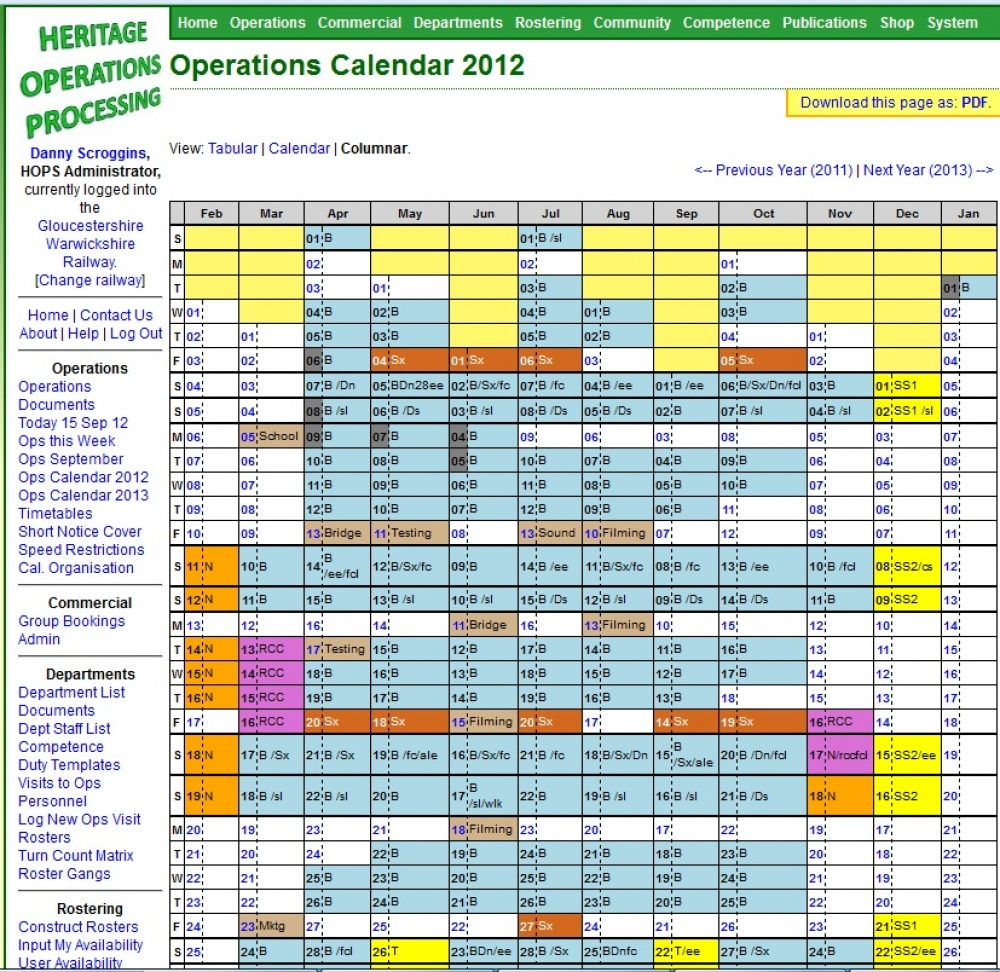
\includegraphics[width=\textwidth]{Figures/hops-operations}
    \caption{The Operations UI as displayed in HOPS.}
    \label{fig:hops} \cite{Hops3}
\end{figure}

The wealth of experience and domain knowledge displayed by the developers of HOPS in their product is clear, as not only does the product go above and beyond the requirements for this project, but it also offered a wealth of functionality, included fully automated rostering functions, but also discussion forums allowing for communication of users, invoicing and financial systems, and even the ability to order, track, and pay for commonly required equipment from HOPS themselves. This functionality appears to be fully customisable, and clients can opt out of functionality that they do not want. The vast majority of HOPS' functionality can be used free-of-charge. \cite{Hops1} \cite{Hops2}

\begin{figure}[!ht]
    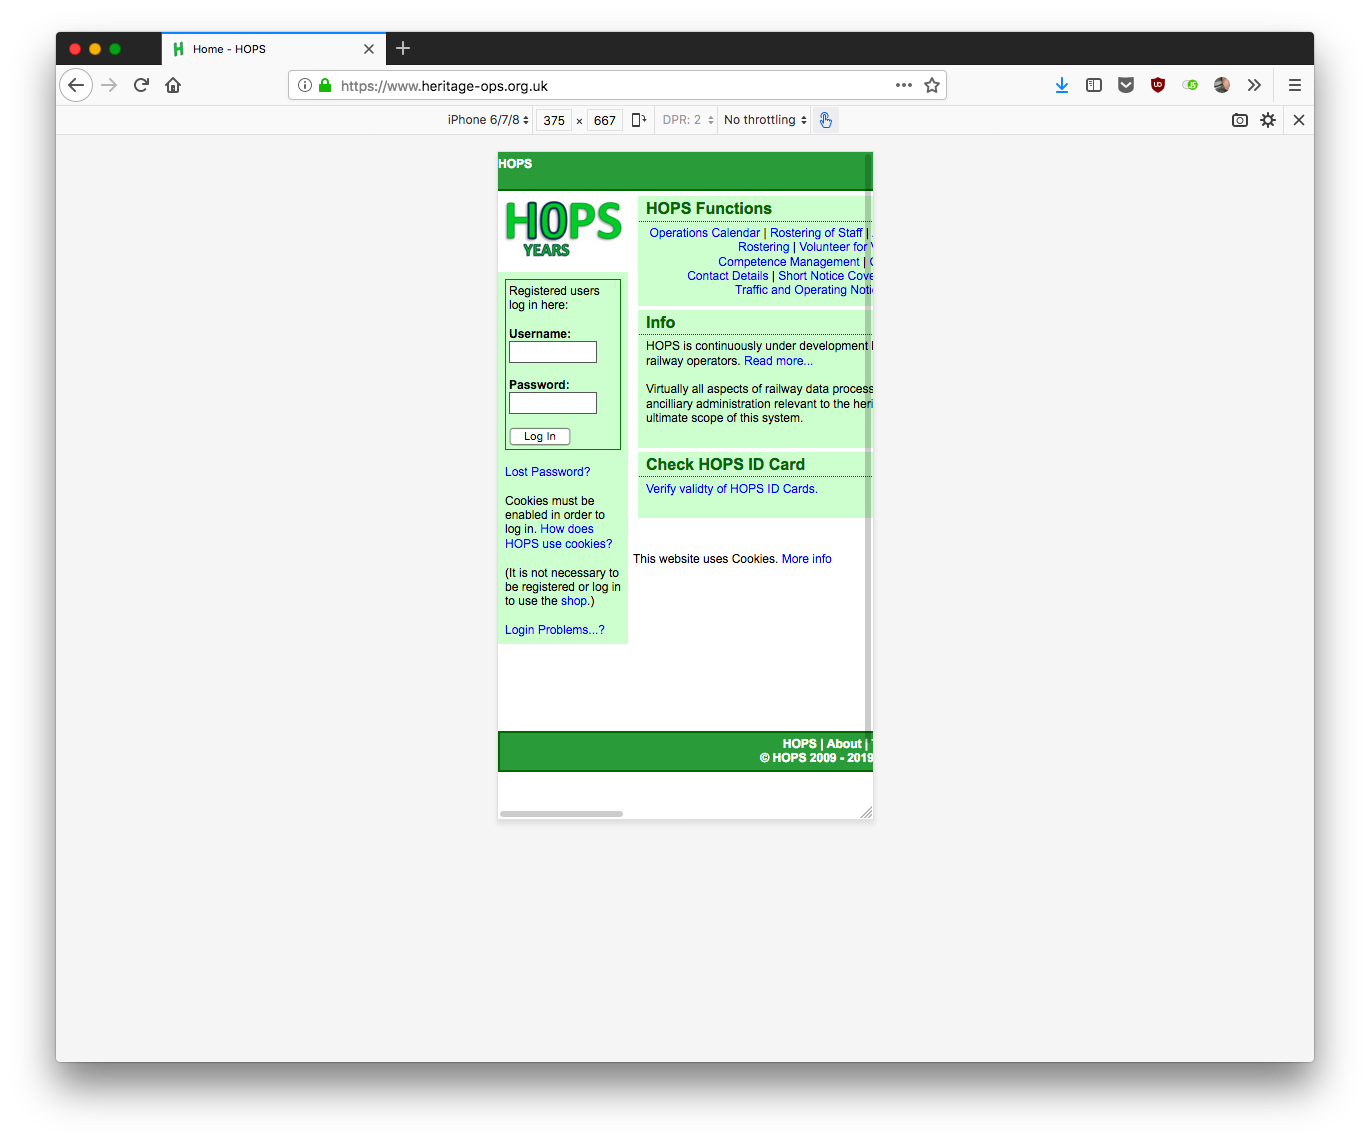
\includegraphics[width=\textwidth]{Figures/hops-unresponsive}
    \caption{HOPS interface is not responsive, as shown in Mozilla Firefox Responsive Design Mode.}
    \label{fig:hops2}
\end{figure}

While HOPS does fulfill the customers requirements almost in full, the interface is visibly complex and difficult to use. Oral conversations with the client revealed that they are well aware of HOPS, but the difficulty in using the interface is a put off for the majority of volunteers, and as a result they resort to using manual spreadsheet solutions as shown in Appendix \ref{Example Timetable}. In addition, HOPS is not responsive, and does not resize itself properly in order to operate in smaller viewports, such as that of a smartphone or tablet. This would require some redesign of the web application front-end and the inclusion of media queries in order to rectify. \cite{6976522}

\subsection{Three Rings}

Three Rings is an online volunteer management system that is entirely run by volunteers, and is at this time of writing used by prominent charities such as The Samaritans, Macmillan Cancer Support, and Citizens Advice. \cite{3r1} It was founded by Dan Q whilst volunteering for Aberystwyth Nightline in 2002, a student-run listening service that catered for the needs of students at Aberystwyth University. \cite{Q1} \cite{AberNL1} In addition, Three Rings has a flexible pricing system, whereby smaller charities and helplines are charged very little, as low as £40 a year, expanding to £600 for nationwide charities - the fee expected is derived from an organisation's annual turnover and volunteer count. \cite{3r4}

\begin{figure}[!ht]
    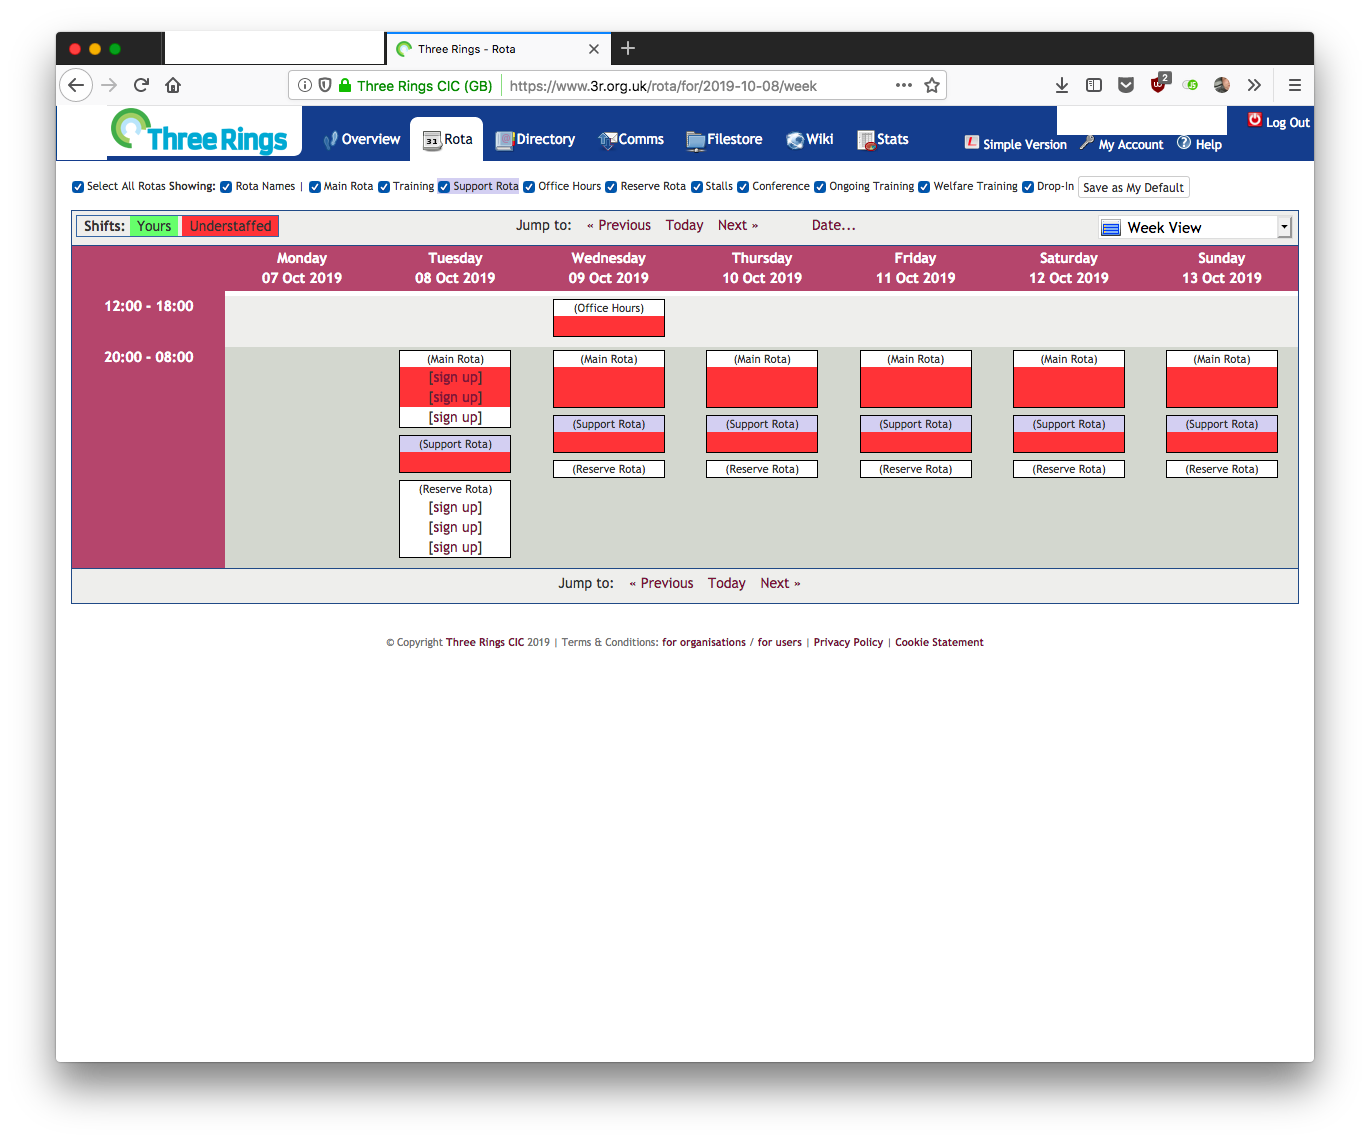
\includegraphics[width=\textwidth]{Figures/3r}
    \caption{Three Rings interface as seen on a desktop web browser, with confidential data redacted.}
    \label{fig:3r}
\end{figure}

Like HOPS, Three Rings is centred around rota functionality that allows for different kinds of shifts to be defined, and users can view and modify their own information. Resultingly, as the application is also designed and subsequently advertised as a mobile-friendly application, it can be easily utilised on a handheld device, and meets all the customer's requirements. Furthermore, the software includes complex stats reporting and an area for uploading and sharing files, as well as support for algorithmically populating vacant rosters with eligible volunteers. \cite{3r3} \cite{3r2}

Finally, Three Rings was recommended, alongside more rudimentary freeware solutions such as Google Calendar, by Voluntary Action Sheffield in a review of various volunteer shift and rota solutions, described as a 'low cost option with a large range of features.' \cite{SVC1}

\subsection{ABC Roster} 

ABC Roster is a proprietary freeware rostering application that is now used by a wide range of businesses and charitiable organisations that prides itself on being easy to use, 'with a convenient and intuitive way of creating schedules quickly.' It appears to include all required functionality, such as availability management, the ability to email staff, as well as desirable bonus functionality such as the automated production of schedules and exportability. \cite{ABC1}

\begin{figure}[!ht]
    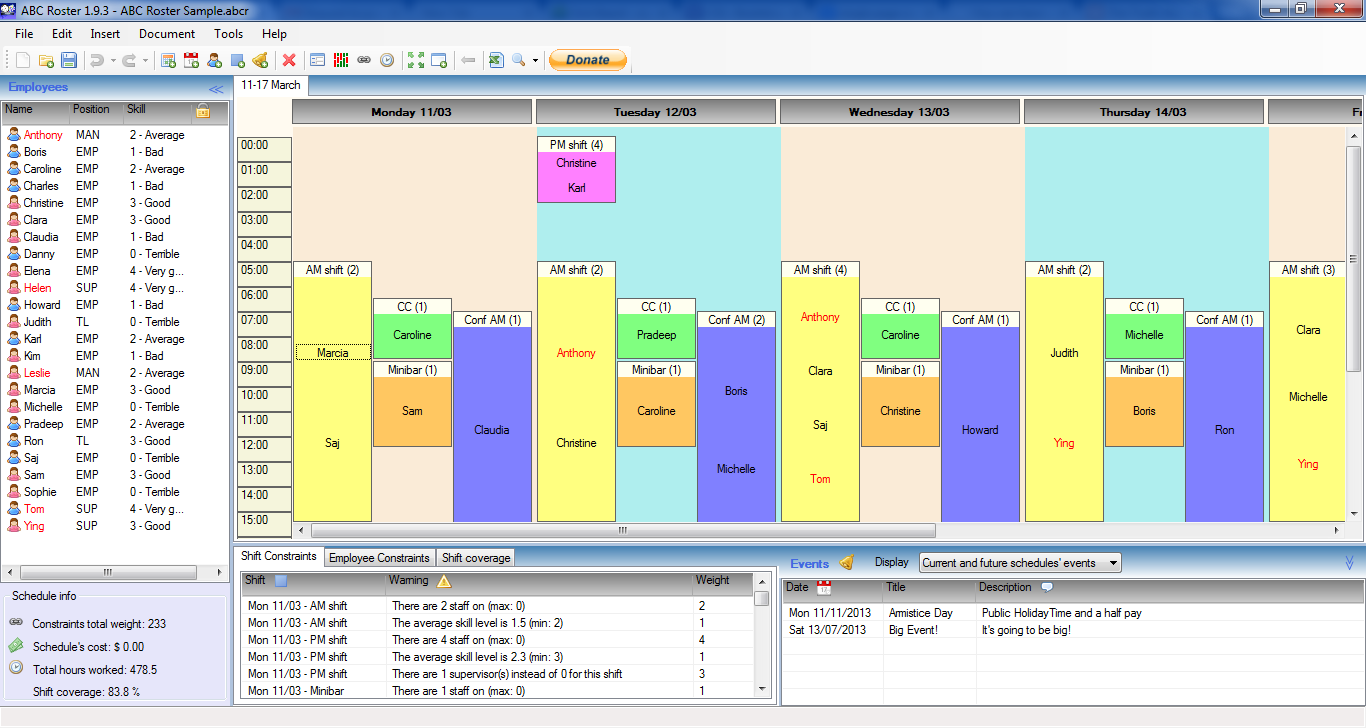
\includegraphics[width=\textwidth]{Figures/abcroster}
    \caption{ABC Roster interface, shown running on Microsoft Windows.}
    \label{fig:abc} \cite{ABC1}
\end{figure}

While a strong contender, with a wealth of functionality and sporting an interface that is straightforward to use, this is a desktop application for Windows, and is both not available for other platforms, such as macOS or GNU/Linux, and is not usable on mobile devices, as it is neither a mobile or web-based application. As the application needs to be able to run on the system requirements outlined on Appendix \ref{Operating Environment}, this is clearly an issue, beyond violating the requirements of a web-based application that can also be accessed on mobile.

In spite of this, there are things that can be taken away from ABC Roster and noted in the construction of a new solution. It's capability to define different roles with differing competencies is noteworthy, as well as the capacity to export rotas into printable form. \cite{ABC1} The software's documentation also provides a detailed insight into the workings of the algorithm responsible for automatically filling in rosters with staff - identifying constraints, weights, and penalties, with an algorithm in likeness to simulated annealing as explored previous:

\[ (3x - 2y) * 4w \]

Let x as the required number of employees; y as the actual number of employees, and w as the constraint weight. The pentalty for satisfied constraints is zero. \cite{ABC2}

\section{Research Conclusion}
While as previously discussed, resolving the NST and implementing an automated rostering solution is beyond the scope of this project, it provides an important insight into the maturity of the computational problem, and importantly the solutions that exist to address said problem, including the software packages in which they are contained. This research is nevertheless a valuable pursuit, as with all agile software projects, there is nothing prohibiting this functionality to become desirable in future revisions, or even as a desired inclusion into an early deliverable. As stated by Ambler, 'project stakeholders have the right to define new requirements, change their minds about existing requirements, and even reprioritise requirements as they see fit.' \cite{Ambler2}

The investigation of existing software solutions has provided a wealth of insight into shared functionality, what solutions do well, and some of their shortcomings that renders them inappropriate. It can be safely concluded from the research that a solution like Three Rings is very ideal for the task at hand, and subsequently this software project should look to emulate its offerings in some form, whilst incorporating doamin specialism demonstrated by a product such as HOPS. In a nutshell, this research has provided valuable insight into what the ideal software solution looks like: responsive and easy to use, with a UI that is similar to the existing calendar / spreadsheet system, and specifically catered for the Corris Railway.

Should this research be continued or expanded upon, it would be ideal to explore even more examples of rostering software, including those used by major corporations and organisations that are not explicitly within the third sector. Furthermore, additional research into implementations of NST solutions is a good direction, so that should this be desired in a future revision of the software, it can be readily and promptly installed.
\chapter{Methodology}

\section{Agile Methodology}
Agile methodologies, a concept solidified in 2001 with the creation of the Agile Manifesto, is the notion of prioritising the delivery of working software and a focus on individuals, including the customer, the developers, and everyone in-between over comprehensive tools, documentation, and rigid plans that are unable to adapt to incoming change. \cite{AgileAlliance1}

As described by Highsmith et al, agile methodologies embrace inevitable change, as opposed to traditional approaches that seek to 'anticipate the complete set of requirements early and reduce cost by eliminating change'. \cite{947100}

\subsection{Adaptation of Scrum}
With prior experience of using agile methodologies in both industry, and in previous academic work, it was quickly decided upon that Scrum would be a suitable candidate framework to adapt and incorporate aspects of to better appropriate it for solo development, and to use it in conjunction with Feature-Driven Development, which would be the primary methodology used.

Scrum is characterised by three primary roles: a Product Owner, a Scrum Master, and a Developer, all of whom carry out unique roles and carry distinct responsibilities within the organisation or development body. In addition, events, such as but not limited to sprints - a fixed unit of time to denote work nominated from a product 'backlog' is to be completed, with regular face-to-face meetings known as daily scrums (or stand-ups), of which the framework derives its name, used to relay progress information and potential setbacks to other members of the team. \cite{Scrum1} In turn, the terminology and analogies used by Scrum, including the name itself, are borrowed from the game of rugby. As stated by Takeuchi et al, 'as in rugby, the ball gets passed within the team as it moves as a unit up the field.' \cite{Hirotaka1}

The main adaptations made to the framework and incorporated into the custom agile methodology used were the assimilation of all roles into a singular role - incorporating the actual development work expected of a software engineer, the responsibilities of a Scrum Master ensuring that the methodology is followed as pragmatically as possible, and the various aspects and duties carried out by a Product Owner, such as communicating and discussing requirements or changes with the customer. \cite{Drumond1}

Secondly and most notably, changes were made to the traditional system of sprints as measurements of time. They were instead simplified into a straightforward timeframe Gantt chart, with date estimates and guidelines that could be modified where necessary, but nevertheless provided an indication of progress and momentum as the ultimate project deadline draws closer. This Gantt chart is available as Appendix \ref{Gantt Chart}.

\subsection{Adaptation of Feature-Driven Development}
\begin{figure}[h]
    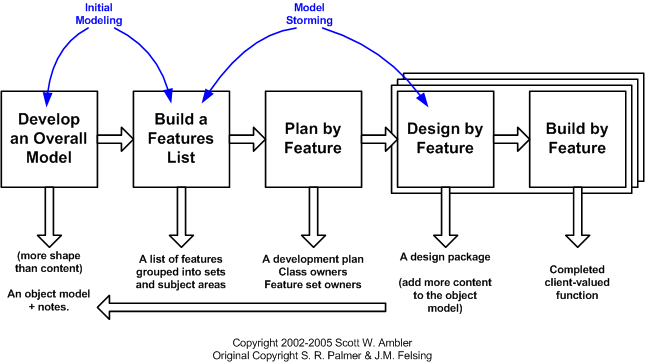
\includegraphics[width=\textwidth]{Figures/fdd}
    \caption{The Feature-Driven Development Lifecycle}
    \label{fig:fdd1} \cite{FDDimage}
\end{figure}

With a well-laid out set of initial requirements defined at the start of the project, Feature-Driven Development was determined to be the most appropriate methodology for use with the project alongside the aforementioned adaptations adopted from Scrum. The concept, consisting of the five processes shown in figure \ref{fig:fdd1} was formulated in 1997 by Jeff Luca in order to aid the software development needs of a bank in Singapore. \cite{Arrk1} These processes can be broken down as follows:

\begin{enumerate}
    \item Develop an Overall Model
    \begin{itemize}
        \item The first step is to produce what is, as described by Goyal, a 'high-level walkthrough of the scope of the system and its context.' \cite{Goyal1}
    \end{itemize}
    \item Build a Features List
    \begin{itemize}
        \item The second process is to produce a hierarchical list of features, typically organised by category. \cite{Goyal1}
    \end{itemize}
    \item Plan By Feature
    \begin{itemize}
        \item The third process determines the order in which features are developed, and typically would also involve the distribution of tasks to team members. \cite{Goyal1}
    \end{itemize}
    \item Design by Feature
    \begin{itemize}
        \item According to Karam, the lead programmer selects what features will be developed next, and a domain expert is expected to begin analysing and 'designing a solution to each feature.' \cite{Karam1}
    \end{itemize}
    \item Build by Feature
    \begin{itemize}
        \item Development work on the nominated features begins, and Karam goes on to further explain, that unit tests should also be produced to ensure that the code produced meets the expectations of the lead programmer. \cite{Karam1}
    \end{itemize}
\end{enumerate}

As a result of the usage of this methodology, with the only notable modification being the consolidation of roles into a single person, a detailed design and feature list derived from the functional requirements more adherent to Feature-Driven Development was produced following an analysis and decision on the technologies that would be used, and is explored in detail in Design.

\section{Version Control}
Version control in software engineering began as the adoption of best practices and techniques that were used in neighbouring fields of industrial manufacturing and design, predominantly for the similarly complex drawings and blueprints of advanced components. \cite{Carstensen1} Today, the vast majority of software projects depend on Git - an open source, distributed version control system (DVCS) that was developed by Linus Torvalds originally for use in Linux kernel development, further popularised by online repository hosts such as GitHub. \cite{LinuxFoundation1}

This project makes use of a Git repository in order to track changes and a historical record that can be reverted back to should code regressions or decision changes be made, as well as keeping an online copy uploaded to the GitHub online repository hosting service so that it is additionally protected against accidental deletion or corruption. The use of Git nevertheless complements agile development even as a solo developer, as Robinson elaborates that 'simply being able to see changes and go back to an earlier version can be a huge help.' \cite{Robinson1}

\section{Supporting Technologies}
This section explores some of the computer applications that were used in order to aid the implementation of the explored hybrid methodology.

\subsection{Discord}
\begin{figure}[h]
    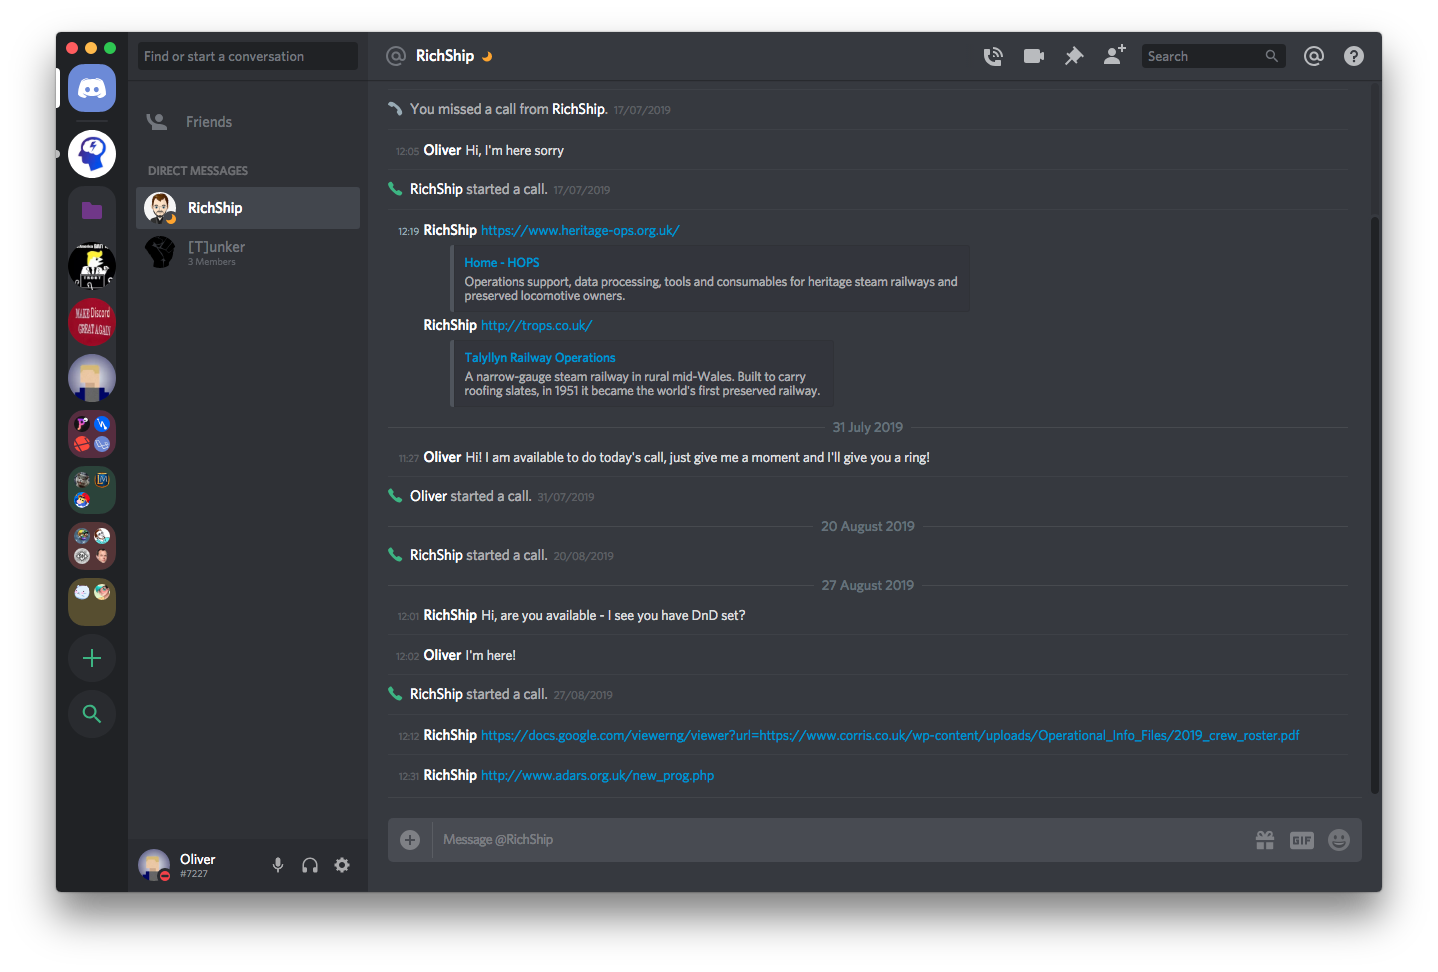
\includegraphics[width=\textwidth]{Figures/discord}
    \caption{A screenshot showing communication history between client and developer, in Discord.}
    \label{fig:discord1}
\end{figure}

Communication, particularly face-to-face communication is an important component of agile methodologies, as described by Inzaurraga as 'making the feedback cycle faster' and 'ensuring development meets the client's expectations'. \cite{Inzaurraga1} The further importance of face-to-face communication is emphasised by Cao et al, who state that such communication 'obviates the need for time-consuming documentation and approval processes' and that it allows 'customers to steer the project in unanticipated directions.' \cite{4420071}

Due to geographical constraints making face-to-face communication difficult, an ideal alternative is audio and video conferencing, which Discord was quickly mutually decided upon to be the facilitatory technology. Discord is a proprietary Voice over IP (VoIP) application available for desktop and for mobile platforms, or usable in a web browser, with functionality including voice and video calling, and importantly, the ability to share a user's desktop view with call participants, a feature known as screen sharing. \cite{Melcon1} Despite the program originally being designed for use by those interested in video games, the application has quickly grown in appeal to other audiences, and competes openly with popular rival messaging and VoIP software, such as Microsoft's Skype. \cite{Giret1}

Weekly voice and video meetings with shared screens were conducted with the client using Discord, as well as facilitating immediate, ad-hoc instant messaging and link sharing whenever necessary, as shown in figure \ref{fig:discord1}.

\subsection{Microsoft Outlook}
\begin{figure}[h]
    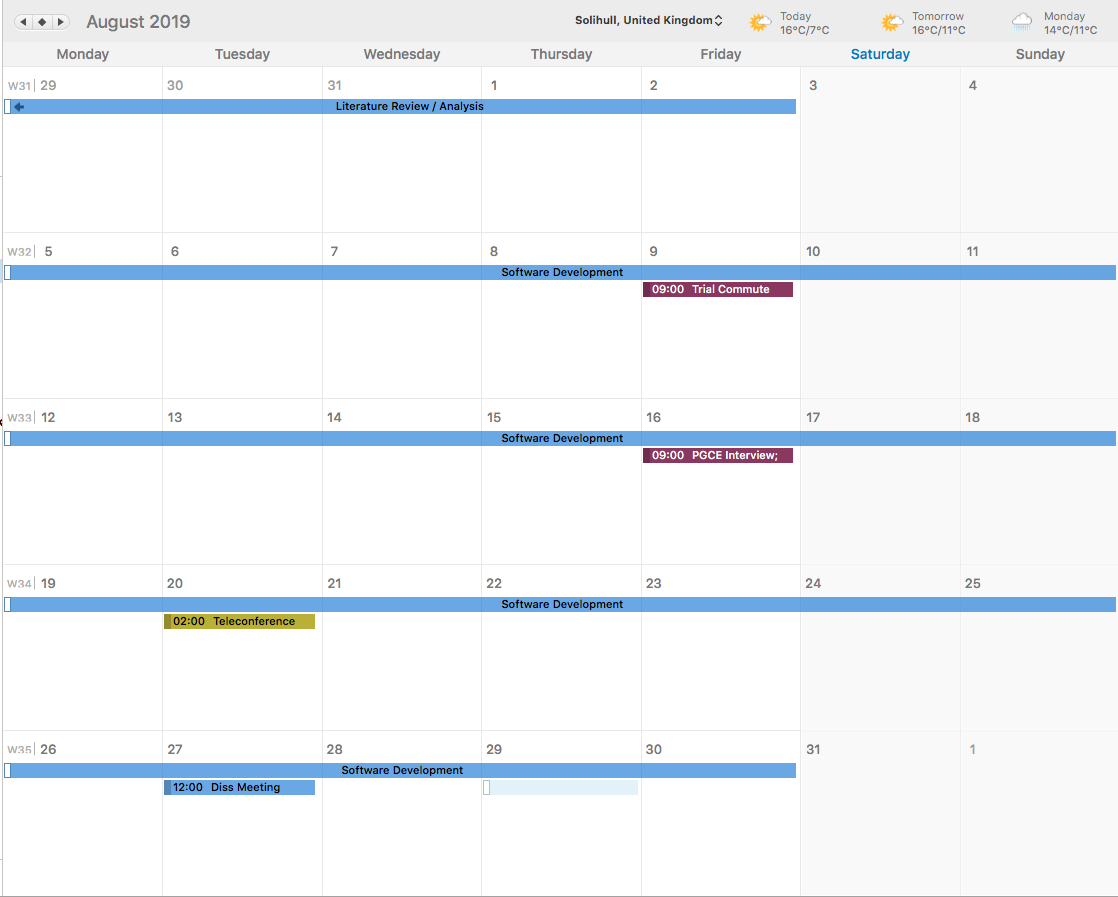
\includegraphics[width=\textwidth]{Figures/outlook}
    \caption{Calendar view in Microsoft Outlook, displaying development time periods.}
    \label{fig:outlook1}
\end{figure}

In order to ensure that development remains disciplined and that the timeframes illustrated in Appendix \ref{Gantt Chart} are maintained as closely as possible, the date durations were added to an appointments calendar within Microsoft Outlook, a popular email, calendar, and newsgroup client developed by Microsoft for Windows and macOS, \cite{Microsoft1} which provided reminders as deadlines approached and as demonstrated by figure \ref{fig:outlook1} were easily viewable at a glance.

While more fitting alternatives for agile software development exist, such as facilities provided by GitHub itself, and also solutions such as Atlassian JIRA, this solution works fine and does not violate the popular KISS (Keep it simple, stupid) principle - a notion that originated in aeronautics, but has since become popular among many branches of engineering, software included. \cite{Branson1}

\subsection{Evernote}
\begin{figure}[h]
    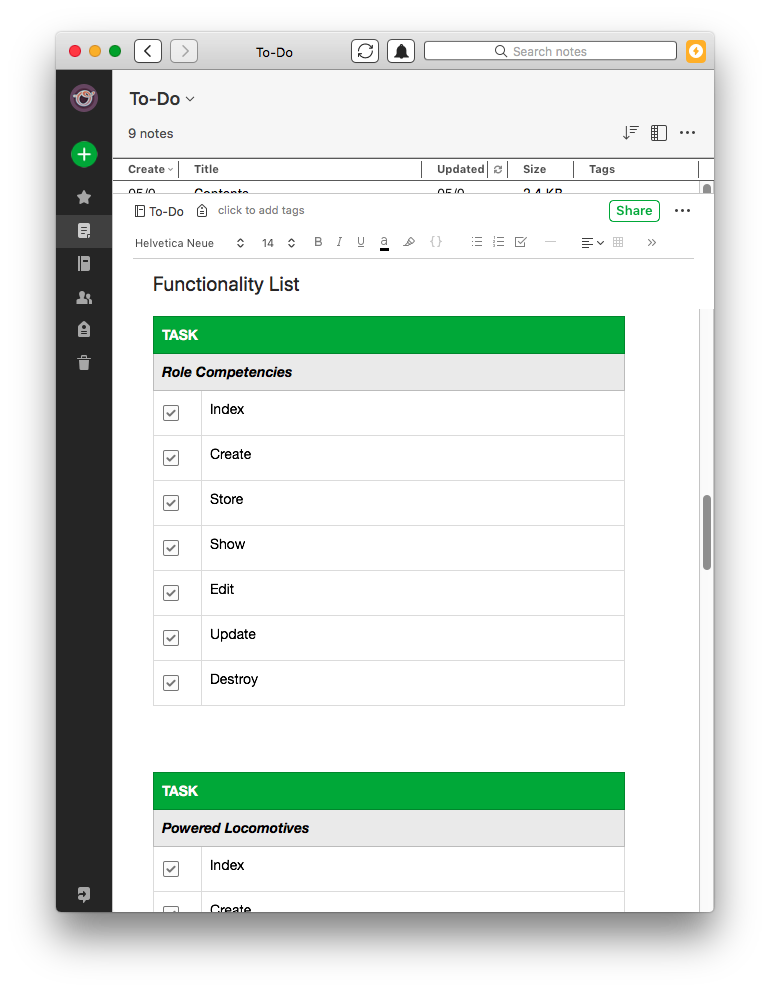
\includegraphics[width=\textwidth]{Figures/evernote}
    \caption{An example of feature checklists displayed in Evernote.}
    \label{fig:evernote1}
\end{figure}

Evernote is a notepad application with a wealth of rich-text formatting features, pre-built templates, and cloud synchronisation support. As it includes ready-to-use templates for to-do lists, complete with clickable checkboxes, it a useful tool for quickly keeping track of functionality that was deemed complete and fully tested. \cite{McCracken1} This proved satisfactory for solo development, although for cooperative undertakings, more specialised tools such as the aforementioned Atlassian JIRA, or the use of a Kanban board would be more optimal.
\chapter{Design}

\section{Analysis of Relevant Technologies}
Determing what programming language(s) and framework(s) to use in a project implementation is an important decision process. A chosen technology must be runnable within the constraints defined in Appendix \ref{Operating Environment}, and ideally should be a technology that the development team, in this case a solo developer, is familiar with as to minimise excessive amounts of time learning.

On the other hand, there is an important balance that must be struck between choosing a tool that is familiar, and that which is most effective, as argued by Vinegar who states that 'writing quality, sustainable software comes second to fiddling with what's sexy'. \cite{Vinegar1}

Ultimately, the languages were refined down to PHP, JavaScript, and Python, as they are all comfortably understood by the developer, appropriate for the task of constructing a full-stack web application, and should run on the designated GNU/Linux system environment without issue.

\subsection{PHP}
PHP, otherwise known by the recursive acronym PHP Hypertext Preprocessor, is one of the most famous and important programming languages on the Internet, originally written in 1994 by Rasmus Lerdorf. It can be used in a procedural or object-oriented style, and is allegedly used on more than 20 million websites today. \cite{Wolfe1}

While PHP can be used on its own to great success, there are numerous frameworks available that build on top of PHP to make it better suited for producing full-stack web monoliths that will likely require the use of the popular Model View Controller (MVC) design pattern. This design pattern is described in greater detail in Design Patterns.

The most popular framework of this nature is Laravel, originally conceived by Arkansas developer Taylor Otwell, who in around 2011 was unhappy with the most popular framework at the time, CodeIgniter. \cite{OBrien1} Today, it features a range of features such as built-in authorisation and authentication, MVC clearly built-in as the core design pattern in mind, security mitigations, and most notably, abstracts a lot of the complex database work that would be required in this project behind an Object-Relational Mapper (ORM) called Eloquent, heavily based on ActiveRecord that is found in Ruby on Rails. This functionality would drastically simply development efforts and reduce the quantity of boilerplate code that would need to be written, when the framework can simply be leveraged instead. \cite{Shah1} \cite{Laravel1}

\subsection{JavaScript (Node.js)}

\subsection{Python}

\subsection{Miscellaneous}

\subsection{Additional Considerations}

\subsection{Conclusion}

\section{Design Patterns}

\section{Data Persistence}

\section{Security Considerations}

\section{Development Environment}

\section{FDD Feature List}

\section{Use Case Design}

\section{User Interface Design}

\subsection{Early Concept Art}

\subsection{Final Iteration}
\chapter{Implementation}

\section{Directory Structure}
The directory structure (for the application only) is defined as follows:

\begin{itemize}
    \item \textbf{app} contains various Laravel application components, such as models, controllers, and policies
    \item \textbf{bootstrap} Framework code used by Laravel to bootstrap the application
    \item \textbf{config} Framework code that define configurations for various Laravel utilities and functionalities
    \item \textbf{database} Database factories, migration definitions, and seeding tools are in this directory.
    \item \textbf{docs} Documentation generated by Sami is stored here. This is explored in more detail in Chapter 7.
    \item \textbf{node\_modules} This contains Node.js dependencies installed by Laravel Mix and are used in development. This is discussed in greater detail in Chapter 7.
    \item \textbf{public} is the front-facing directory containing the application entry-point, as well as compiled assets and images used for social media.
    \item \textbf{routes} HTTP Application routes are defined in the files contain within this directory.
    \item \textbf{resources} Views written in Laravel Blade are kept in this folder, along with stylesheets and scripts that comprise the front-end.
    \item \textbf{storage} Laravel stores log files here, and generated PDF files for download are kept here. A cache for quick loading is also stored here.
    \item \textbf{tests} PHPUnit tests are kept here, and are covered in Chapter 6.
    \item \textbf{vendor} Similar to \textit{node\_modules}, this folder stores PHP dependencies used by Laravel, as well as additional third-party libraries.
\end{itemize} \cite{W3Schools1}

\section{Method of Action}
The Laravel developers acknowledge that having a basic, high-level understanding of how a framework works is important for not only having a basic grasp of how the application works, but also to make 'everything feel less magical'. \cite{Laravel6} This is important as frameworks are characterised by carrying out substantial amounts of work for you, in order to drastically reduce development time and to produce better quality applications, and are generally recommended by the greater web development community. \cite{Mozilla3}

\begin{figure}[!ht]
    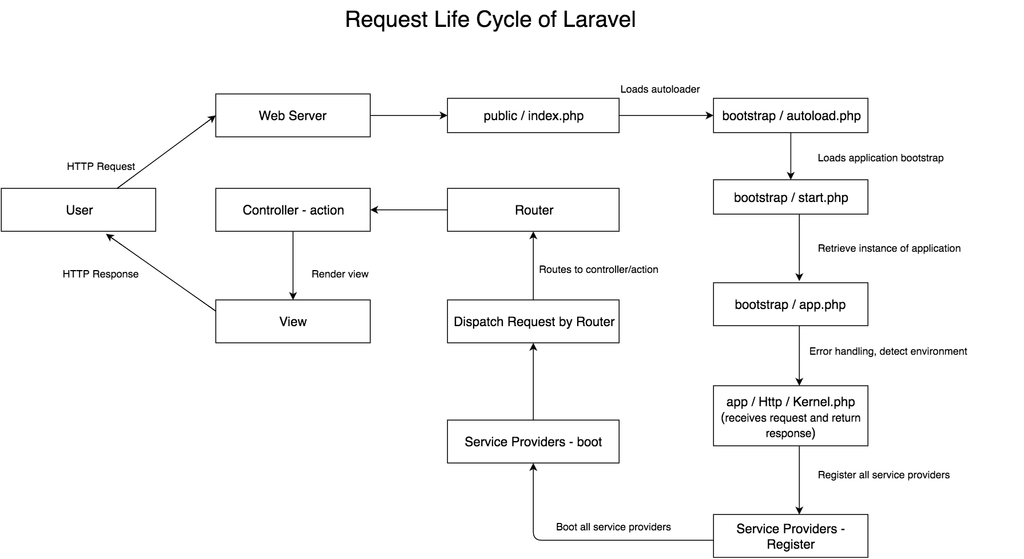
\includegraphics[width=1.0\textwidth]{Figures/laravel-request}
    \caption{Diagram that shows how the Request Lifecycle for the Laravel framework operates.}
    \label{fig:laravel-requests} \cite{Mallow1}
\end{figure}

When a HTTP (Hypertext Transfer Protocol) request is received by the web server by navigating to the \textbf{index.php} file in the \textit{public} directory, the application is quickly bootstrapped, loading all necessary libraries and components by means of the PSR-4 autoload file, which is a widely accepted PHP coding standard and was generated by Composer, the PHP package manager when the application was first installed. \cite{PSR1} From here, the application can determine how to 'route' the request based on route definitions and the URL (Uniform Resource Locator) path, delegating actions to the appropriate controllers and their models defined in those definitions, before passing data to a view, and returning it to the user. \cite{Laravel6} According to Stauffer, Laravel's approach 'brings your ideas to reality with no wasted code' and 'modern programming standards.' \cite{LaravelUp1}

\section{HTTP Routes}

\begin{figure}[!ht]
    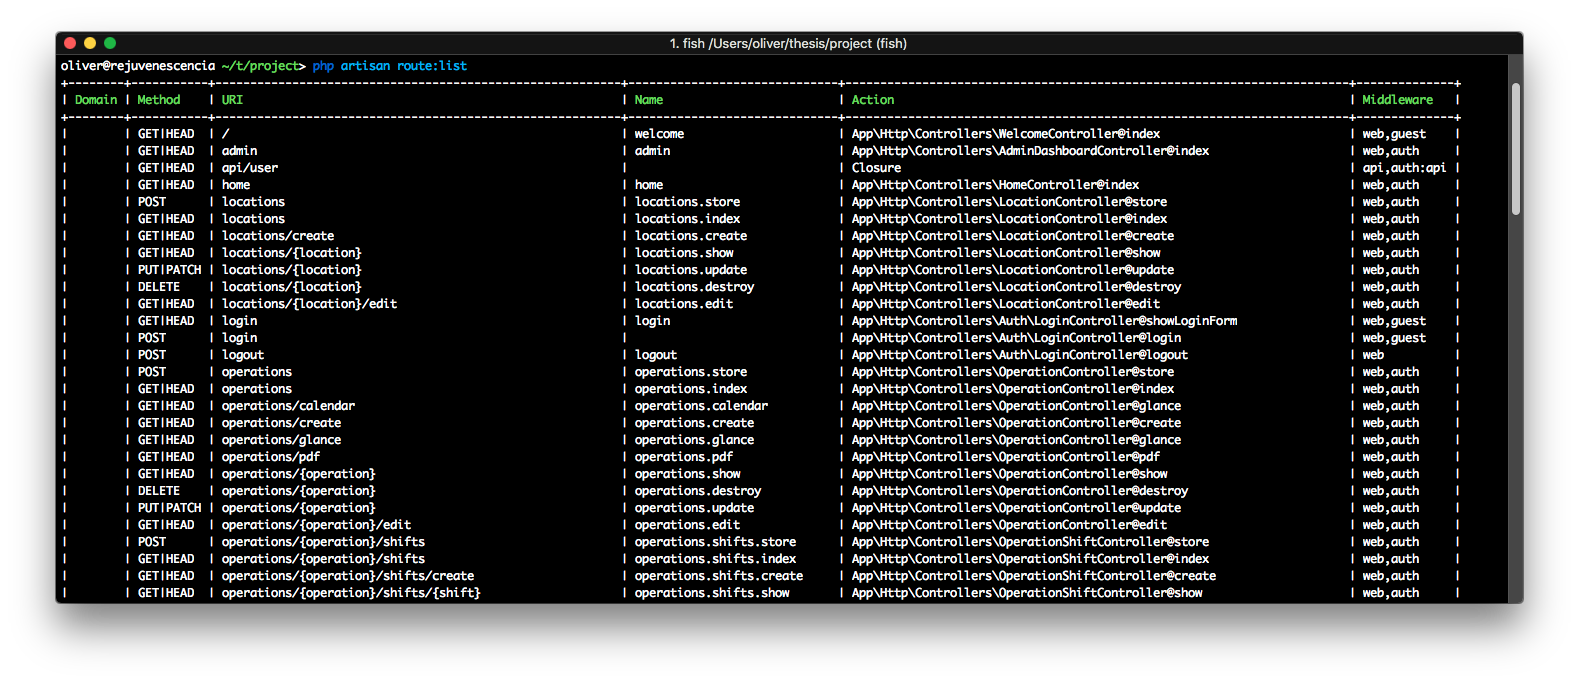
\includegraphics[width=1.0\textwidth]{Figures/routes}
    \caption{A print out of HTTP routes defined within the application, their corresponding URLs, associated controllers and methods, and HTTP actions.}
    \label{fig:methods}
\end{figure}

The controllers for each resource (i.e. users, operations) as well as individual webpages uses a RESTful (Representational State Transfer) architecture, and have methods that correspond to the CRUD verbs - create, read, update, and delete. There are also additional methods that help facilitate the CRUD operations, such as 'show' for viewing individual entries, and 'edit' to display a form in order to modify an existing record. Different actions may expect different HTTP requests, such as GET, POST, PATCH, and DELETE respectively. Each action, whether viewing one's own profile, editing a user's profile, registering for a shift, or deleting an operation, are all represented by their own route within the application, including custom defined routes that do not correspond to CRUD, such as those used for (de)registering to an operation. \cite{Laravel7} \cite{7539825}

\section{Models and Relationships}

\begin{figure}[!ht]
    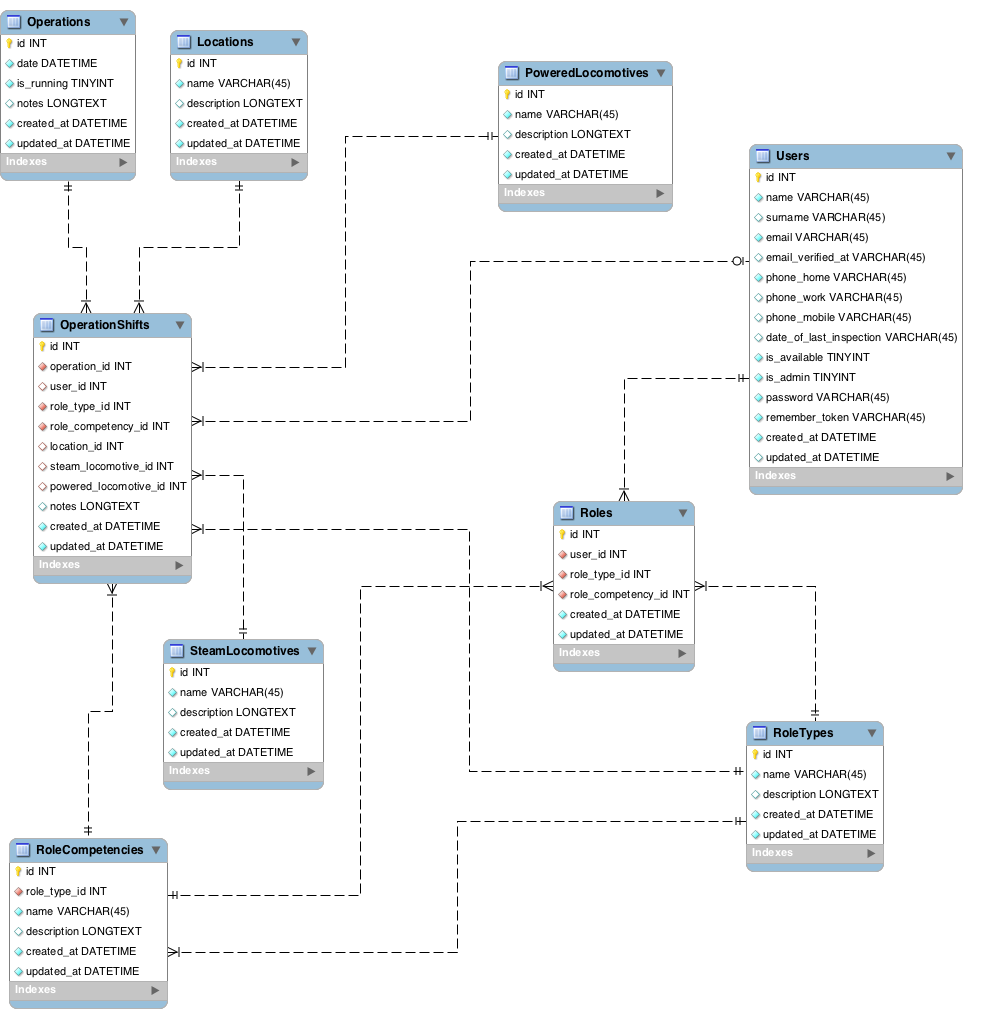
\includegraphics[width=1.0\textwidth]{Figures/Models}
    \caption{UML diagram showing the relationships between database tables and their structure. The relationships are defined by their Eloquent relationships.}
    \label{fig:relationships}
\end{figure}

Database models define their column names and data types within migration files, alongside foreign keys, their references, and any constraints. As shown by Figure \ref{fig:relationships}, many of the tables belong to shifts, as each shift can have corresponding vehicles associated with it, a designated location, a required role and competency level, as well as the volunteer that is assigned to that volunteer, which is of course null when the shift is vacant.

\section{Views and Laravel Blade}

Controller methods, as part of their response to the user's request will return a view that can be populated with data processed or retrieved, such as returning the current resource object for display when viewing an individual item, like a role type. Laravel uses a language called Blade for its templating engine, which allows for reusable front-end code, and more legible syntax for inserting data into views or extending existing template files than using raw PHP alone, though vanilla PHP script is nevertheless supported and will be interpreted all the same. \cite{Laravel9} \cite{Underwood1}

An example of a data being passed to a view can be seen in the following code, that is taken from the controller for operations, where all operations retrieved from the database (by Eloquent) are injected into the view as an argument, to be parsed and displayed there:

\begin{lstlisting}[language=PHP, breaklines]
    public function index()
    {
        $operations = Operation::orderBy('date', 'desc')->paginate(3);
        return view('operation.index', compact('operations'));
    }
\end{lstlisting}

The name of the view to be rendered by Laravel is 'operation.index', which will now have access to the contents of \texttt{\$operations}. In the following snippet of Blade code, you can see the contents of this variable being iterated through and printed in tabular form, as well as the usage of vanilla PHP script where it has been deemed necessary:

\begin{lstlisting}[language=HTML, breaklines]
    <tbody>
    @foreach ($operations as $operation)
        @php
            $operationDate = \Carbon\Carbon::parse($operation->date);
        @endphp
        <tr>
        ...
        </tr>
        ...
    @endforeach
    </tbody>
\end{lstlisting}

\section{Users}

\begin{figure}[!ht]
    \centering
    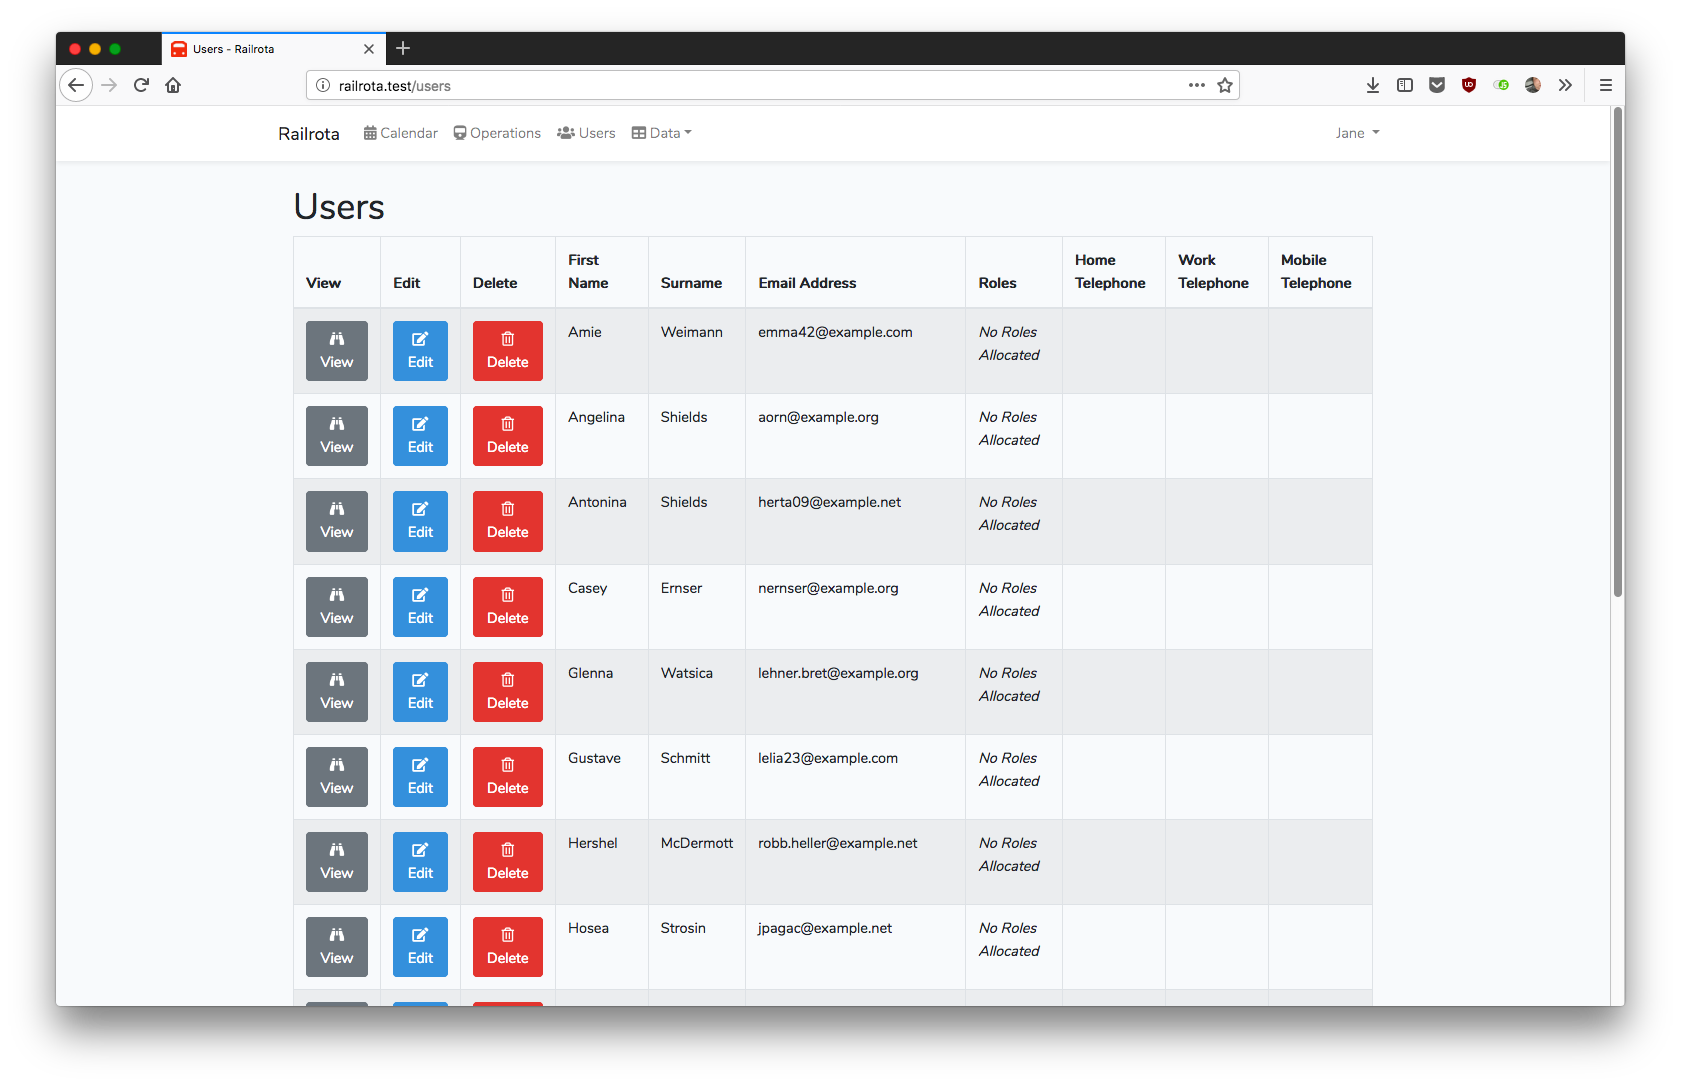
\includegraphics[width=1.0\textwidth]{Figures/screenshot-users}
    \caption{Screenshot of the Users interface within the application.}
    \label{fig:users}
\end{figure}

All volunteers are users within the application, with users that have access to administrative privileges being denoted by a boolean true value in \textbf{is\_admin}. Users can modify a subset of their own information, but are unable to assign themselves roles or privileges, or modify a date value indicating the last time they were inspected.

\begin{figure}[!ht]
    \centering
    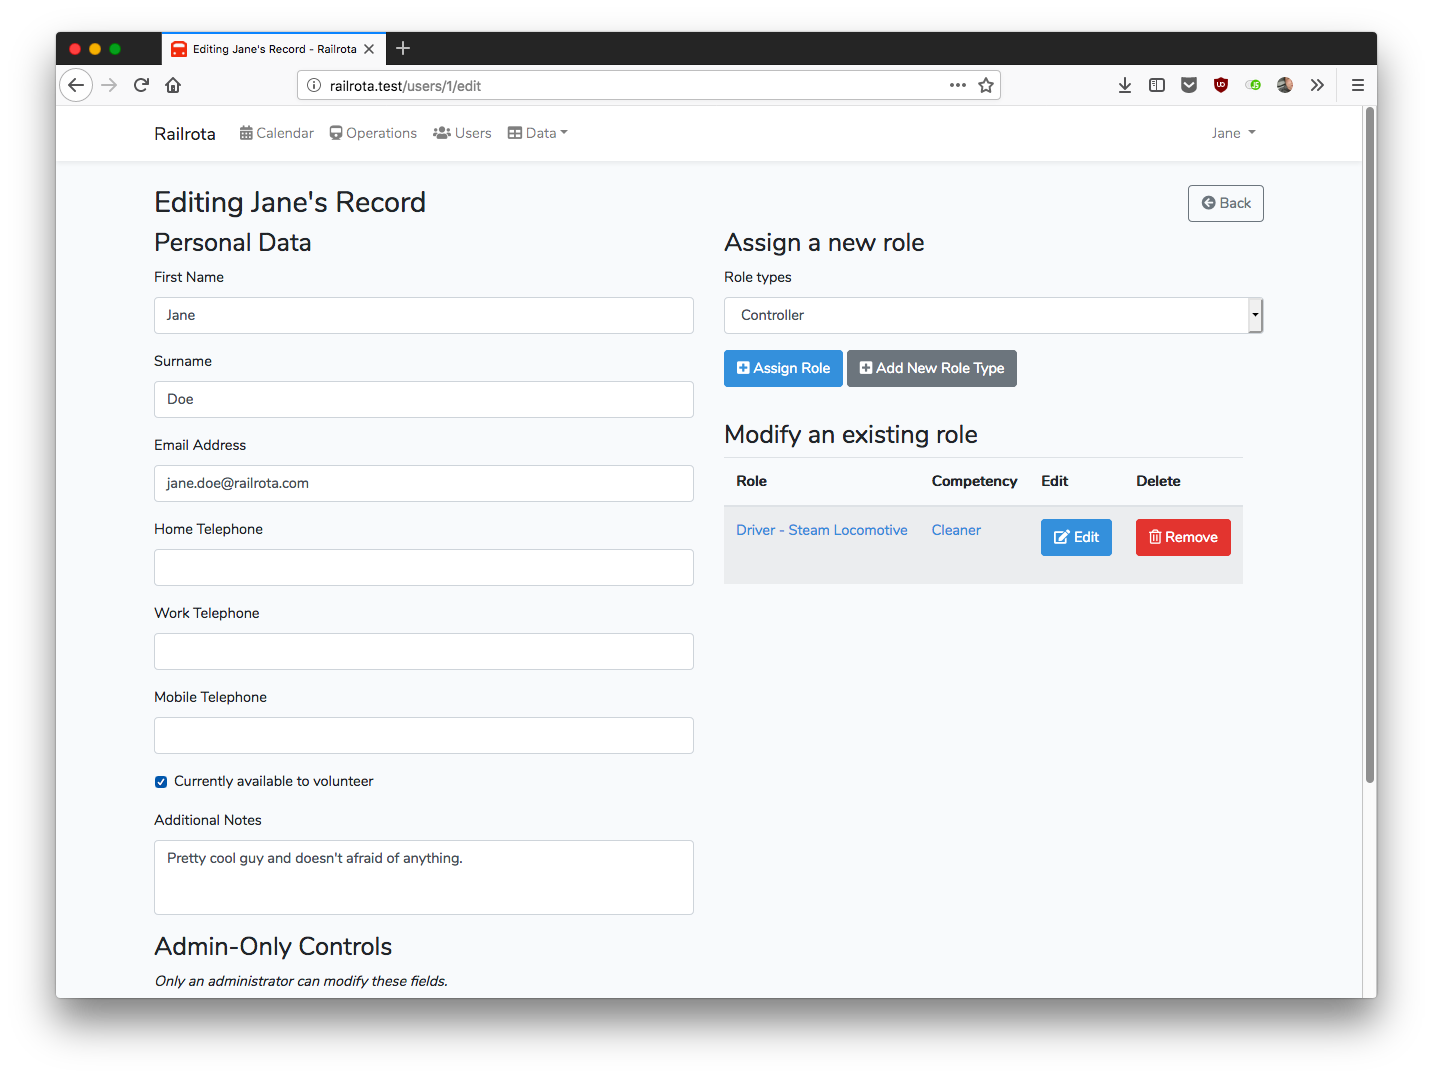
\includegraphics[width=1.0\textwidth]{Figures/screenshot-edit-user}
    \caption{Screenshot of the Edit User interface, as seen by an administrator.}
    \label{fig:users-edit}
\end{figure}

The following destroy CRUD method in the User controller, demonstrates how after checking the policies that the current user is authorised to delete a user (so is an administrator), it checks first whether they are attempting to delete themselves, which is understandably undesirable behaviour, and redirects back with an error message if this is the case. Otherwise, the \textbf{delete} Eloquent method is called on the user object, and it is deleted from the database; redirecting back with a success notification. The User object is resolved from the unique ID in the URL. \cite{Laravel7}

\begin{lstlisting}[language=PHP, breaklines]
    public function destroy(User $user)
    {
        $this->authorize('delete', $user);

        if ($user->id === Auth::id()) {
            flash()->error('You can\'t delete yourself!')->important();
            return redirect()->back();
        }

        $user->delete();
        flash()->success("{$user->name} has been deleted successfully!")->important();
        return redirect()->route('users.index');
    }
\end{lstlisting}

\subsection{Authentication}
Authentication functionality can be scaffolded seamlessly by Laravel by issuing the \texttt{php artisan make:auth} command at on the command line, and provides all the necessary registration, login, and password reset functionality - and automatically ties this into the User model.

By declaring routes within the authentication middleware group as the following code demonstrates, Laravel will ensure that a user is authenticated in order to access any of the routes contained therein, otherwise redirecting back to the login page. \cite{Laravel8}

\begin{lstlisting}[language=PHP, breaklines]
    Route::group(['middleware' => ['auth']], function() {
        Route::resource('users', 'UserController');
    }
\end{lstlisting}

\subsection{Authorisation and Policies}
Authorisation - determing who can and who cannot access resources or carry out certain actions is determined by classes known as policies within Laravel - where authorisation logic is stored. \cite{Larashout1} In this application, a policy is necessary wherever there are actions that users and administrators have different levels of access to, such as being able to create roles, operations, or modify user data.

A corresponding method is typically called in a controller's respective policy (i.e. UserController will have a matching policy called UserPolicy) and within the controller action itself, the appropriate method for that action is passed as an argument, alongside the currently authenticated user object, like thus:

\begin{lstlisting}[language=PHP, breaklines]
    $this->authorize('create', $user);
\end{lstlisting}

This calls the corresponding create method in its policy file, which will return either true for successful authorisation and allowing the remainder of the controller method to execute. Otherwise, the action is prevented. A call to this method absolutely must exist for any authorisation to occur, regardless of whether there is a corresponding policy class to the aforementioned controller and model. The corresponding 'create' policy method in the UserPolicy file is as follows:

\begin{lstlisting}[language=PHP, breaklines]
    public function create(User $user)
    {
        return $user->isAdmin();
    }
\end{lstlisting}

This simple but effective method calls a custom method on the model itself that returns whether or not the attribute \textbf{is\_admin} on the currently authenticated user is true or not. If the value isn't truthful, then execution halts as authorisation has subsequently failed.

\section{Role Types}

\begin{figure}[!ht]
    \centering
    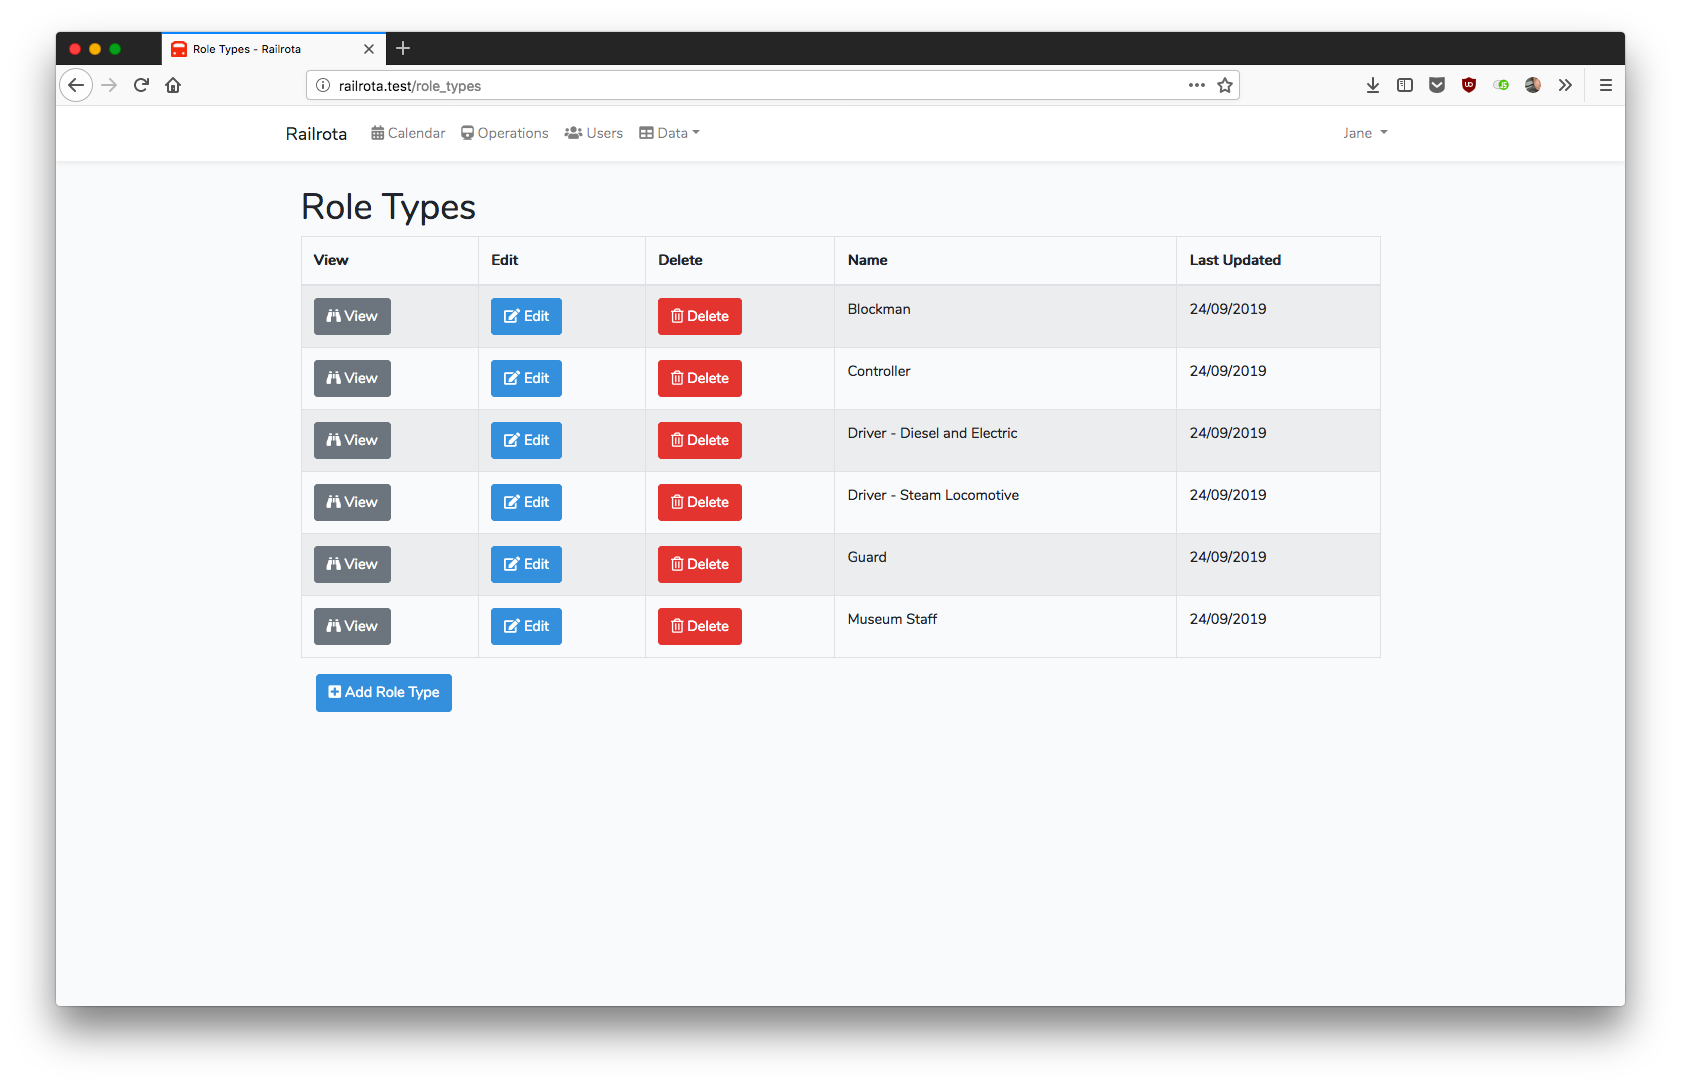
\includegraphics[width=1.0\textwidth]{Figures/screenshot-roletypes}
    \caption{Screenshot of the Role Types interface within the application.}
    \label{fig:roletypes}
\end{figure}

In order to volunteer for a shift, a user must have the relevant role type that is also shared by the shift. For example, a shift might have a \textit{Blockman} vacancy available, but in order to volunteer for the role, they need to have that role themselves. Role types are treated as resources with CRUD routes, and can only be modified in any form by administrators.

Role types are not hardcoded into the system, and are their own database table, although a list of defaults is defined in the source code that can be used during initial setup, and consist of the following roles: 

\begin{itemize}
    \item Controller
    \item Guard
    \item Blockman
    \item Driver (Diesel/Electric)
    \item Driver (Steam)
    \item Museum Staff
\end{itemize}

Additional role types can be added to the system to accommodate any future needs of the railway, or existing ones may be modified or deleted as necessary.

\section{Role Competencies}

\begin{figure}[!ht]
    \centering
    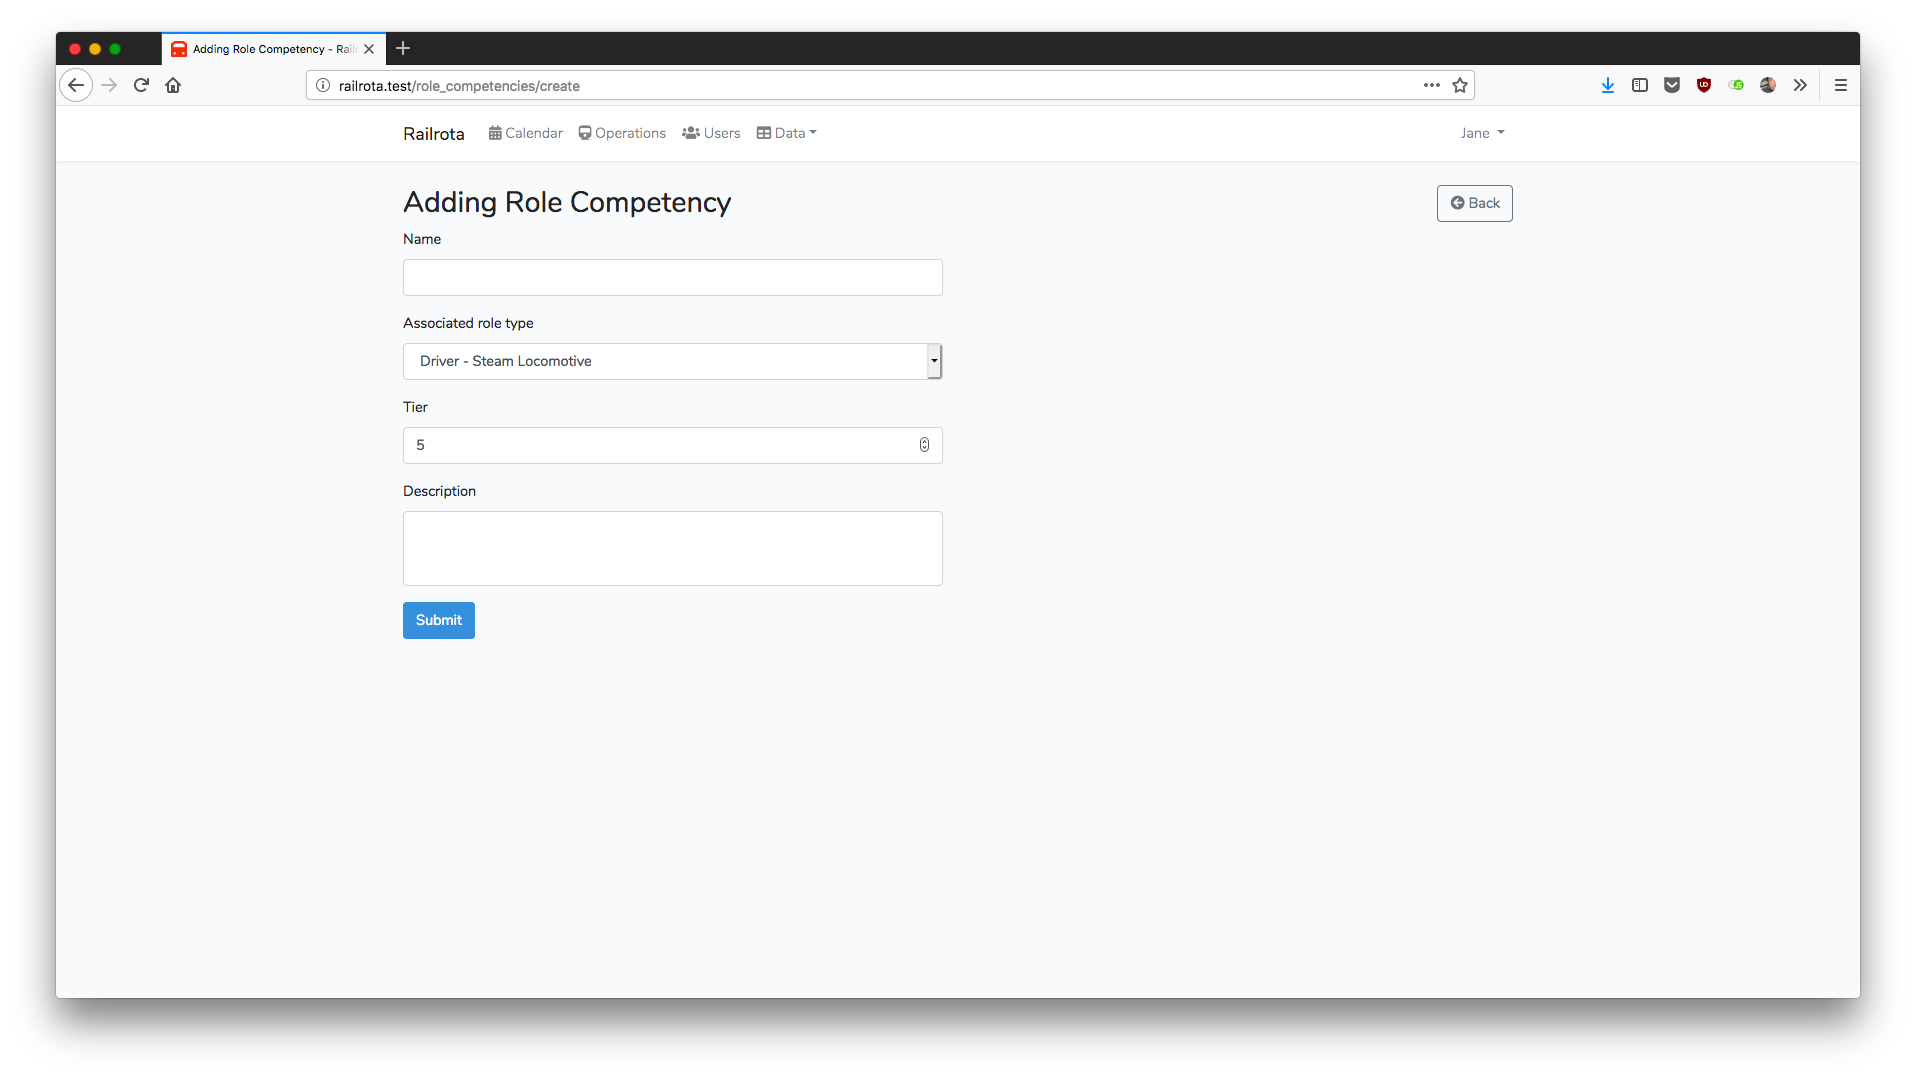
\includegraphics[width=1.0\textwidth]{Figures/screenshot-competency-create}
    \caption{Screenshot of an administrator adding a new competency level to the a driver role.}
    \label{fig:competencies-create}
\end{figure}

Each role can have multiple competency levels, each with their own tier between 1 and 10. Those with a competency in a specific role can volunteer for shifts equal or lesser to their numerical tier. 

For example, if there is a Blockman Shift requiring at least a Trainee, which have a numerical tier of 1, then those with Passed (2) or Examiner (3) can also sign up for the same work. If the shift required someone with Passed (2) level, then a Trainee (1) would not be able to register for it.

Each of the default role types have predefined default competencies also, but additional competencies can be added and those existing may also be modified. Furthermore, the numerical tiers are not unique, so multiple competencies for a role may share the same tier. Shifts can also not have tier requirements set, and can therefore be met by any level, including if a user does not have a competency level defined for whatever reason.

This algorithm that ensures that competency levels are met is explored in more detail in the Operations and Shift subsection.

\section{Roles}

A role type and role competency is linked to a user by means of a role - which can be viewed as properties of a user, as users can have multiple roles each with their own role type and role competency.

As they are used akin to a pivot table, tying information on the aforementioned tables together, there are no forms to directly create them, and the necessary controls to do so are only visible to an administrator on the respective user's edit UI, as shown by figure \ref{fig:users-edit}.

\section{Locations and Locomotives}

\begin{figure}[!ht]
    \centering
    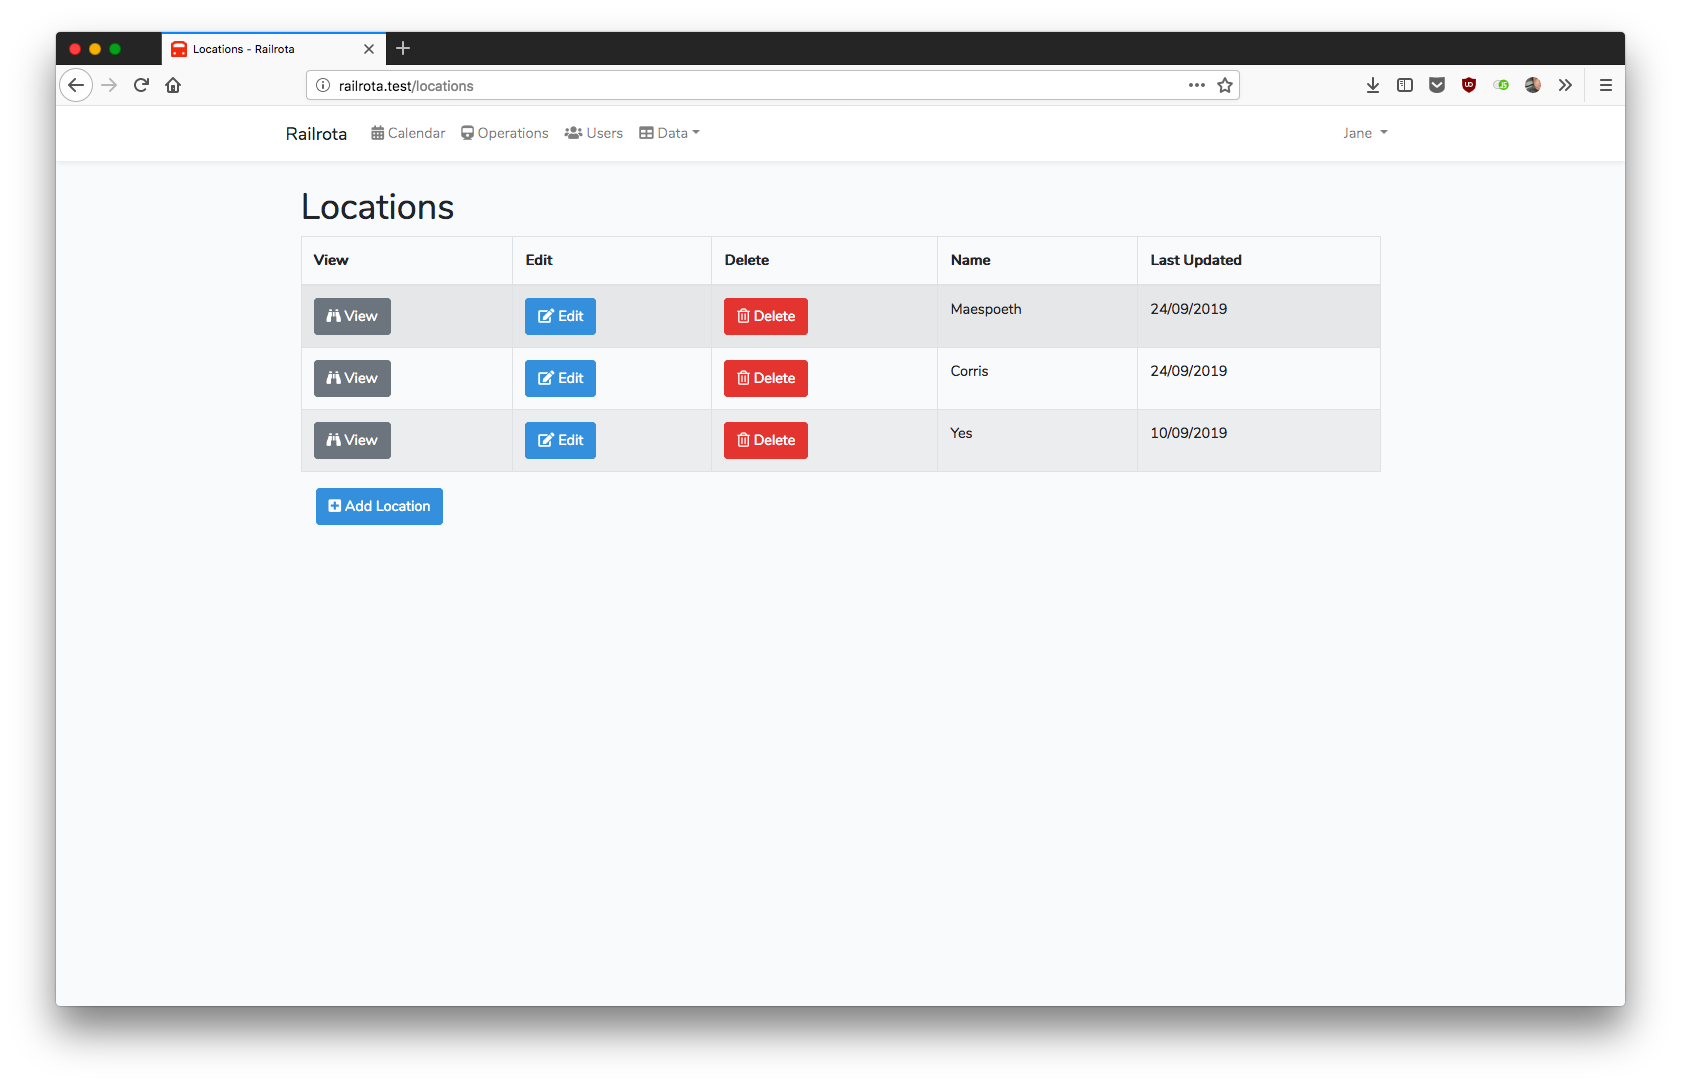
\includegraphics[width=1.0\textwidth]{Figures/screenshot-locations}
    \caption{Screenshot of locations being listed within the application, which is viewable by all users.}
    \label{fig:locations}
\end{figure}

Locations and two types of Locomotives, both Steam and Diesel/Electric are all individual tables in the database but have been grouped for the sake of brevity, as they all function in an identical way, with the only difference being that they have different default values that can be used during initial set up. The information is minimal - the name, an optional description, and timestamps.

Shifts can have optional location information, providing information to users where a shift is located (i.e. what station or railway, or some other geographical location) and if it involves a vehicle, such as a steam locomotive, which one. These resources can only be created or manipulated by administrators, but users can view information about them in the same way they may view other resource data.

When deleting any of these nullable resources, shifts that point to affected table entries will also be nulled.

\section{Operations and Shifts}

\begin{figure}[!ht]
    \centering
    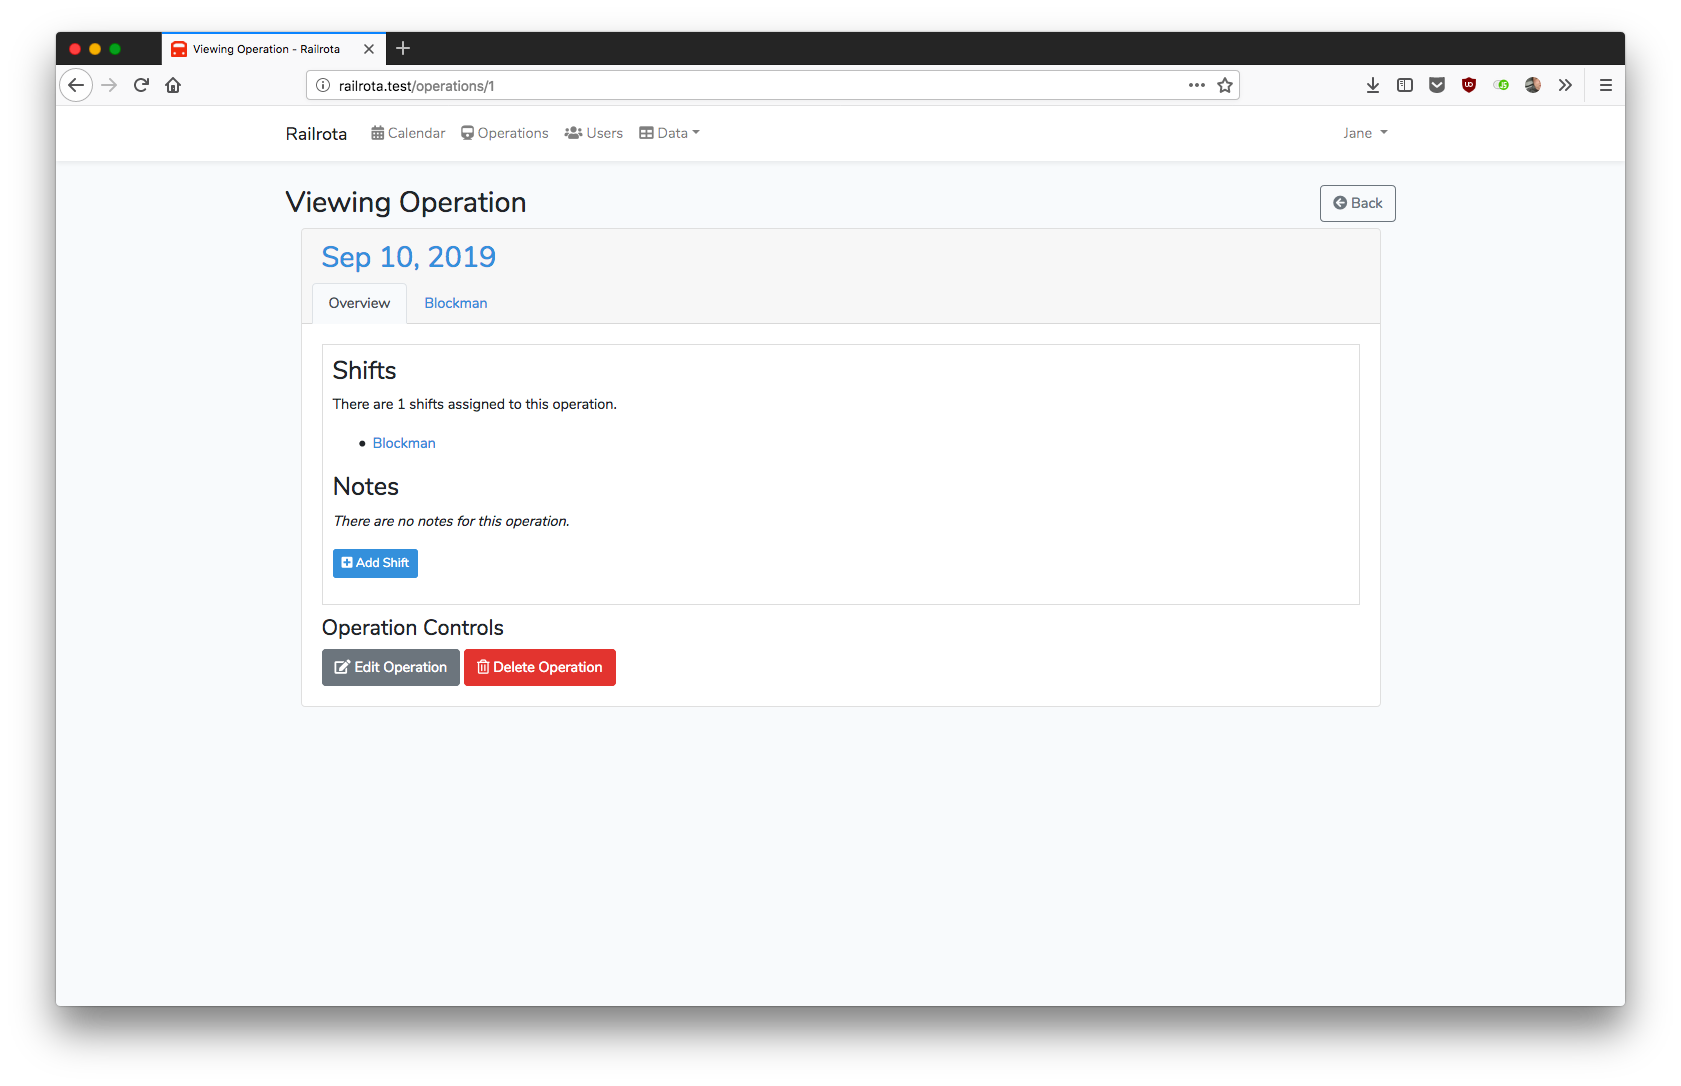
\includegraphics[width=1.0\textwidth]{Figures/screenshot-operations}
    \caption{Screenshot of the operations interface, containing one shift and administrative controls.}
    \label{fig:operations-screenshot}
\end{figure}

Operations are each individual day where the railway will be operating, and each operation can have an unlimited amount of shifts. A shift is a specific volunteering vacancy, with its only requirement being the role type, i.e. what kind of work is required for that shift. Additional information such as location, locomotives, and competencies can also be specified, but are optional. Users can be manually assigned to shifts on creation, such as if an administrator knows in advance that a volunteer is to staff a certain shift, which can, with warning, override any typically enforced role requirements.

In a nutshell, an operation can be thought of as a workday, with each vacancy therein being an individual shift. This system is inspired by the exisitng system showed in Appendix \ref{Example Timetable} and additional domain knowledge examined from research into the HOPS platform. \cite{Hops2} If the operation is declared closed for whatever reason, such as understaffing of critical volunteers, it is impossible for users to sign up for shifts.

\begin{figure}[!ht]
    \centering
    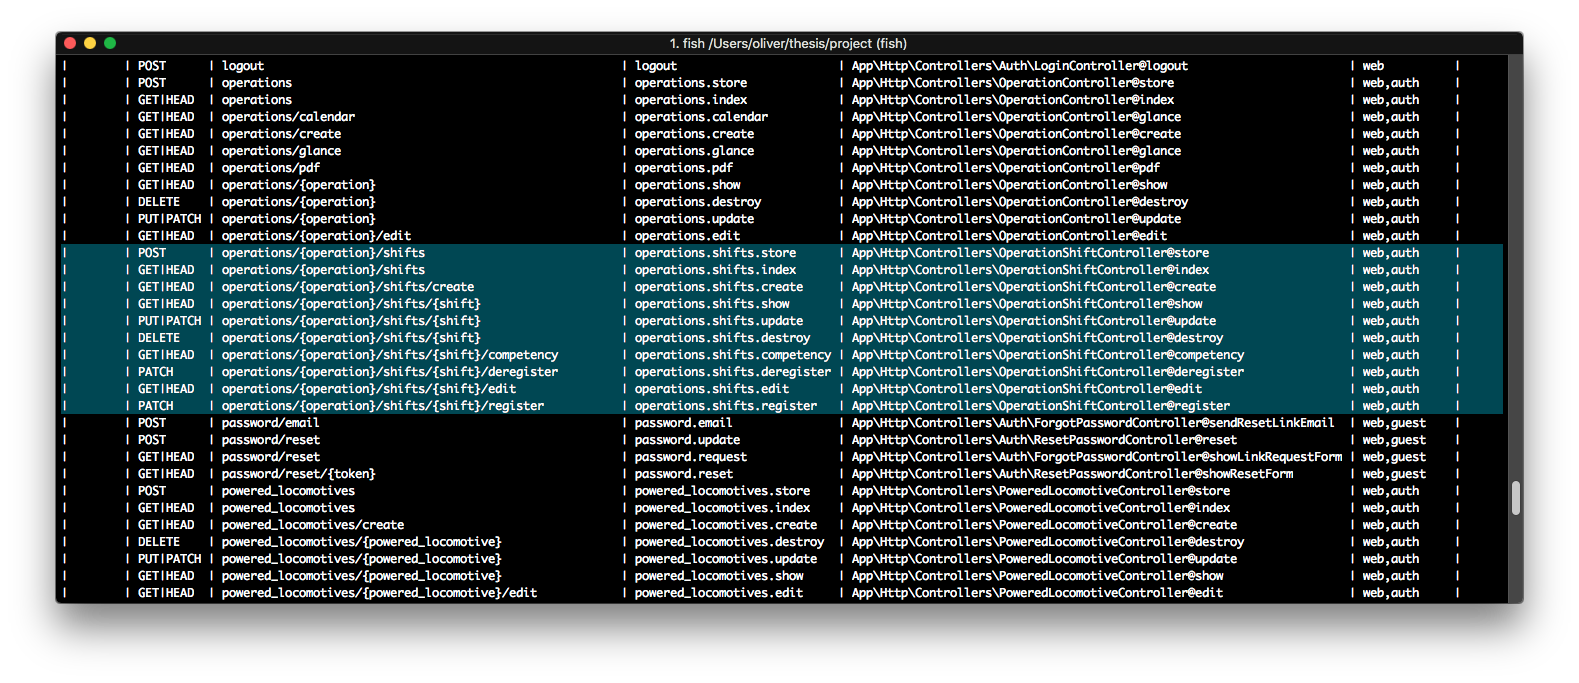
\includegraphics[width=1.0\textwidth]{Figures/nested-components}
    \caption{Screenshot showing how nested components (operations and shifts) appear within Laravel.}
    \label{fig:nested}
\end{figure}

All operations can be viewed in a reverse-chronological, paginated view, or individual operations and their shifts can be viewed independently. This is one of three primary ways of viewing shift availabilities and their information, designed to be a more modern, bespoke solution for navigating data in line with early concept artwork. It is important to note that shifts are a nested resource of operation - shifts cannot be viewed individually as they are instrinsically dependent on their operation. How this is represented in Laravel is shown in figure \ref{fig:nested}. If an operation is deleted, shifts associated with it are also deleted to prevent the occurance of orphaned shifts within the database.

Whilst adminstrators have complete control over operations and shifts and as aforementioned, can manually assign users to shifts, regular users are expected to sign up for shifts that they are capable (in terms of role and role competency) to do. This is referred to internally as 'registering', with pulling out of a shift and leaving it vacant as 'deregistering'.

Whilst deregistration is relatively straightforward and generall risk-free, registering for a shift is complex and carries out substantial amounts of validation checks to ensure that a volunteer is eligible to do so. First, the currently authenticated user is checked for administrative privileges. If they have them, they are able to bypass all further checks, as they are expected to ensure that rules are enforced themselves and not be confined by the rules of the system. 

\begin{lstlisting}[language=PHP, breaklines]
    public function register(Operation $operation, $id)
    {
        ...
            $roleCheck = Role::where([
                ['user_id', '=', Auth::id()],
                ['role_type_id', '=', $operationShift->role_type_id]
            ])->first();
            
            if (is_null($roleCheck)) {
                flash()->error('You do not have the required role type.')->important();
                return redirect()->back();
            } else {
                if (!is_null($operationShift->role_competency_id)) {
                    if ($roleCheck->role_competency->tier < $operationShift->role_competency->tier) {
                        flash()->error('You do not have a sufficient competency / grade tier.')->important();
                        return redirect()->back();
                    }
                }
                if (!is_null($operationShift->user_id) && $operationShift->user_id !== Auth::id()) {
                    flash()->error('This shift is not vacant.')->important();
                    return redirect()->back();
                }
            }
        }
        ...
    }
\end{lstlisting}

Otherwise, the user is first retrieved from the database and checked to see if the user has a role associated with them with the required role type. If they do not, then an error is displayed and the user is redirected back. The next check ensures that, if the shift has a competency requirement specified, that the user meets that requirement by having a tier level that is not less than required, and failure is met with the same fate.

Lastly, the system checks that the shift has not already been filled and the user is erronously attempting to overwrite another volunteer's place in the system. While the interface would normally not allow for this, the check has been put into place to protect against malicious or accidental data submission, such as from an old or manipulated form.

With these checks complete, the remainder of the method continues executing, and data is saved to the database using Eloquent, before redirecting the user to a view and alerting them of their success.

\section{Calendar View}

\begin{figure}[!ht]
    \centering
    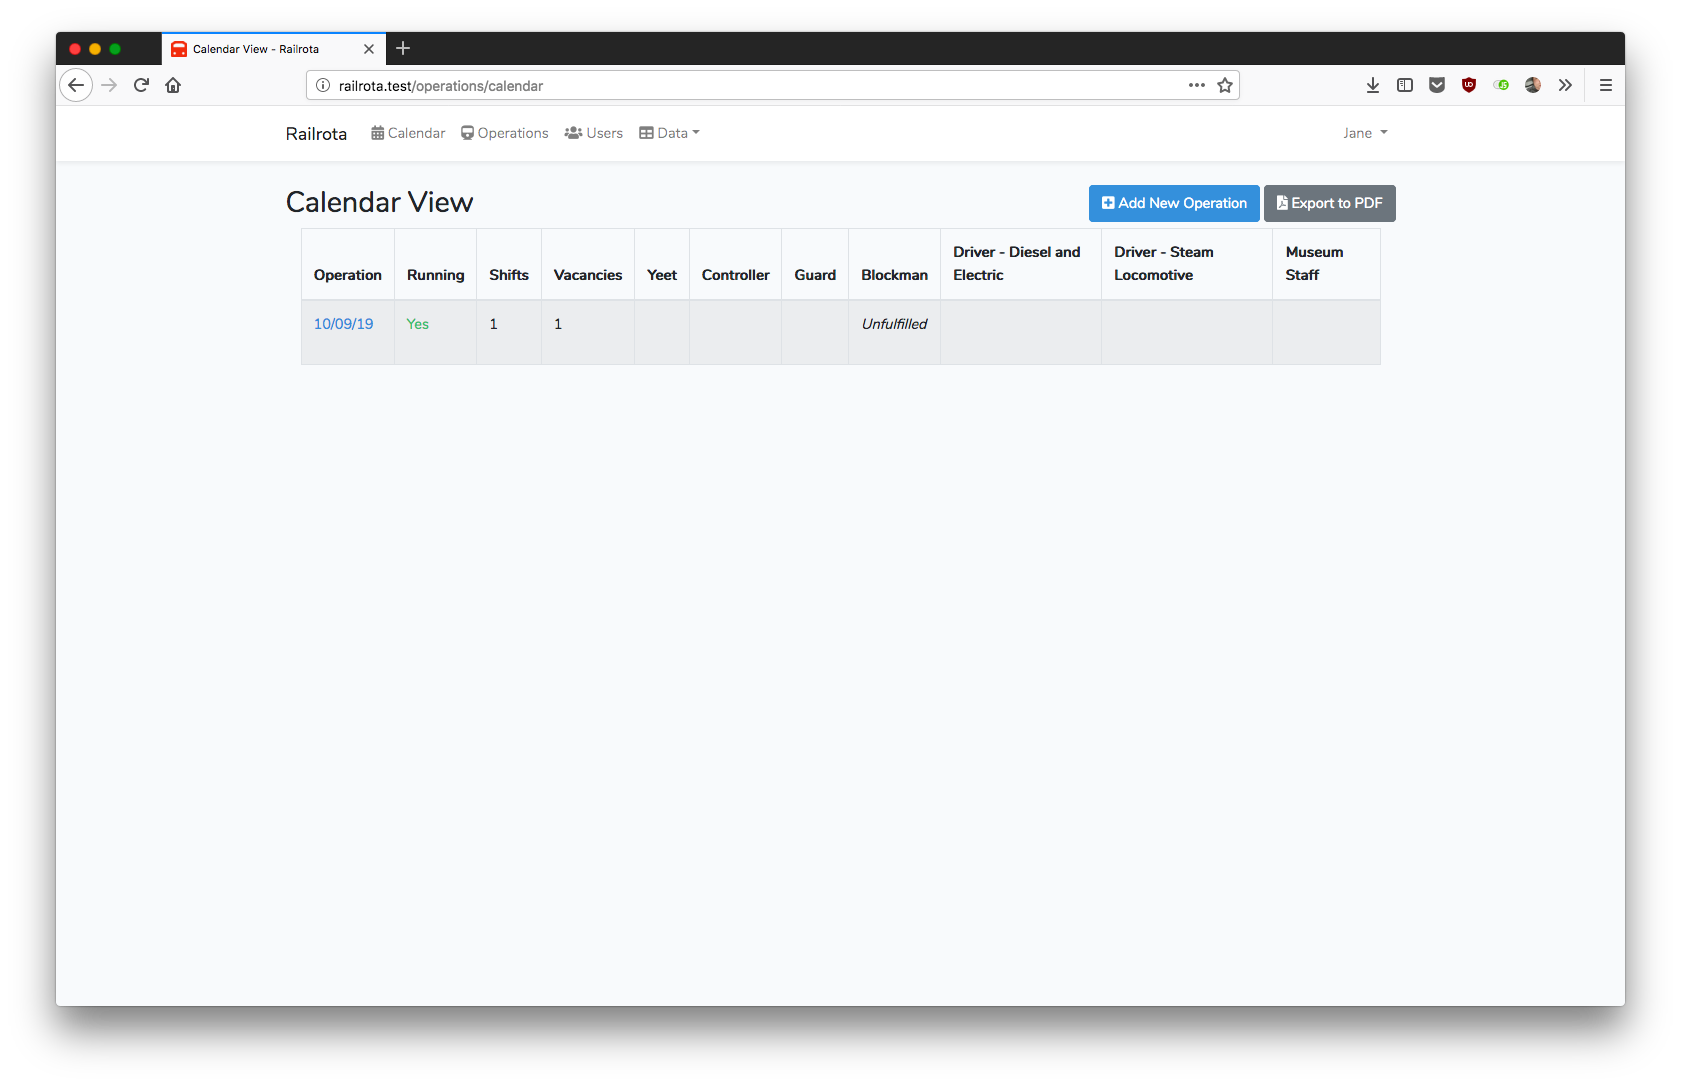
\includegraphics[width=1.0\textwidth]{Figures/screenshot-calendar}
    \caption{Screenshot showing the calendar view, with one operation containing a vacant shift.}
    \label{fig:calendarview}
\end{figure}

Originally coined 'at a glance' view, or just 'glance' view, this functionality was intended to mimic the existing calendar used in Appendix \ref{Example Timetable} to make the transition to the new application easier, and to provide a straightforward means of being able to view vacancies and volunteer staffings en masse. This went through numerous iterations, following multiple rounds of feedback with the customer, before reaching its current phase, reflected in figure \ref{fig:calendarview}.

Information is spread horizontally, where each operation will contain the names, or a registration link, for vacancies of any shifts running of each type. If there are multiple shifts with the same role type, they will co-exist responsively within the same table field. Historic vacancies - vacancies that went unfilled the day following the operation are labelled as 'unfulfilled'.

\section{PDF Export Functionality}

\begin{figure}[!ht]
    \centering
    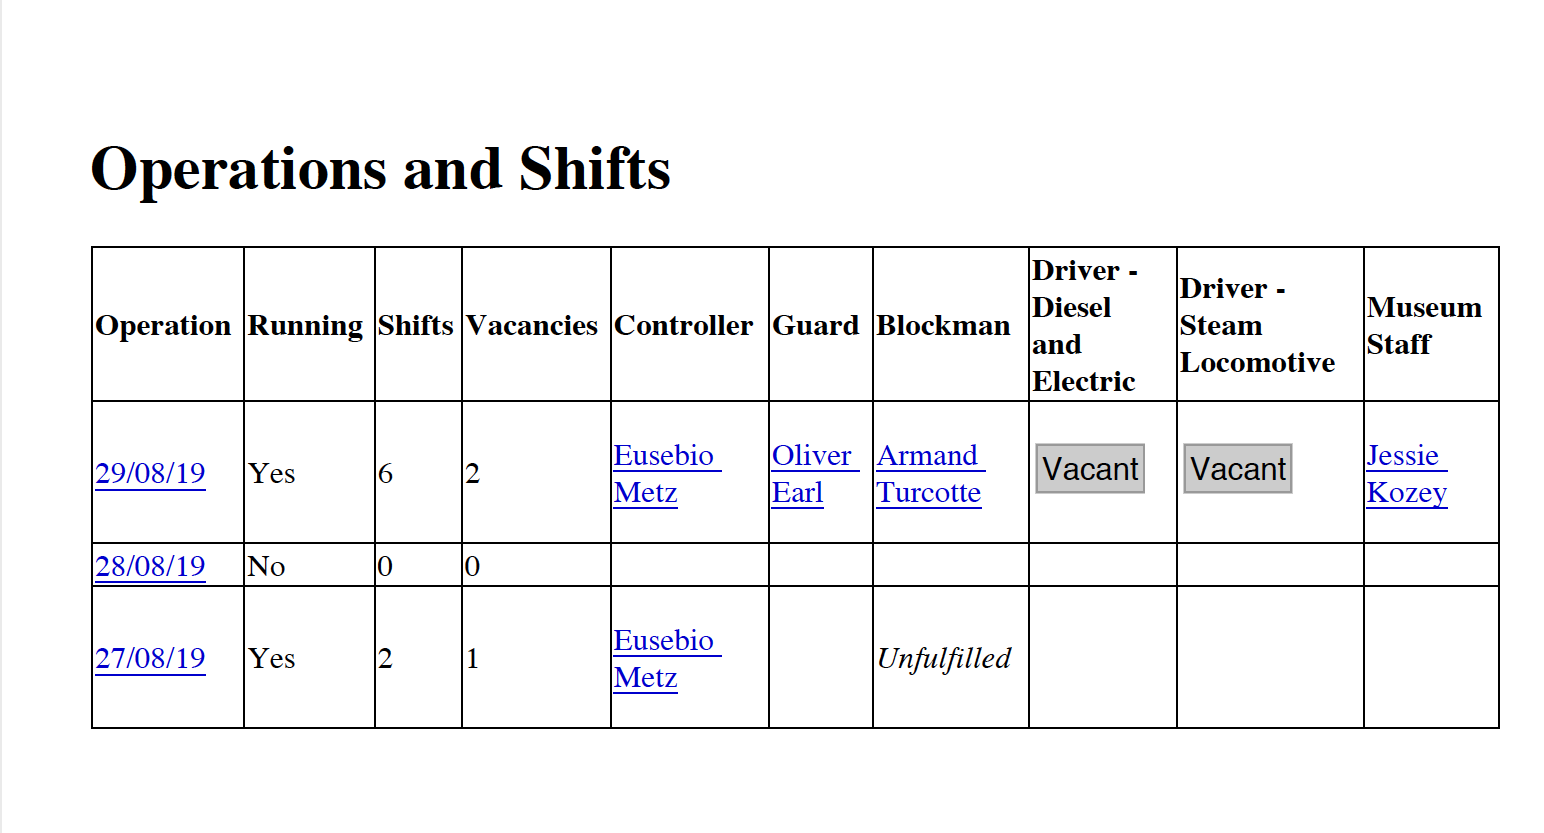
\includegraphics[width=1.0\textwidth]{Figures/screenshot-pdf}
    \caption{Screenshot of an exported PDF containing operation and shift data.}
    \label{fig:pdf}
\end{figure}

As the previous system was purely spreadsheet based, it was a simple task to print and distribute copies of the current timetable to volunteers for their convenience. While this is not mandatory functionality requested by the user, it was deemed important enough for inclusion in order to better bridge the gap in workflow between systems. 

The system works by using a PHP library known as DOMPDF, which renders HTML (Hypertext Markup Language) and CSS (Cascading Style Sheets) of webpages into PDF documents. Getting this set up to work with the Laravel framework would have been particularly challenging, if not for a pre-existing open source Laravel wrapper called laravel-dompdf developed primarily by Dutch developer Barry vd. Heuvel. This made installation incredibly straight forward, and the wrapper provided the necessary Laravel facades and configuration modules to quickly access the library's features and integrate it into the framework. \cite{dompdf1} \cite{Heuvel1}

A custom route was defined to generate PDF documents, which calls a pdf method in the operations controller:

\begin{lstlisting}[language=PHP, breaklines]
    public function pdf()
    {
        $operations = Operation::orderBy('date', 'desc')->get();
        $roleTypes = RoleType::all();
        $filename = Carbon::now()->format('ymd') . '_operations.pdf';
    
        $pdf = \App::make('dompdf.wrapper');
        $pdf->loadView('pdf.operations', compact('operations', 'roleTypes'));
        $pdf->save(storage_path() . '/' . $filename);
    
        return $pdf->download($filename);
    }
\end{lstlisting}

The workings of this method are rudimentary to understand, as most of the heavy lifting is done behind the scenes by the library. First, all operations are retrieved in descending order by leveraging Eloquent and stored within \texttt{\$operations}, and all role types are similarly retrieved and stored within another variable. A filename string is built by using the Carbon datetime library, which is included with Laravel, and concatenating '\_operations' to the end of it. This produces a filename in the format of '20190127\_operations.pdf'.

With this necessary information obtained, a new instance of laravel-dompdf is instantiated, and is requested to load a particular view that utilises basic, print-appropriate layout and styling, and injecting the previously retrieved data to be parsed by Blade. Once done rendering, a copy of the generated PDF file is saved in the Laravel storage directory. Lastly, the file is presented to the user for download.

\section{Additional Webpages}
There are three additional webpages, in addition to those used by application resources, and those used for authentication (i.e. login, register).

\begin{figure}[!ht]
    \centering
    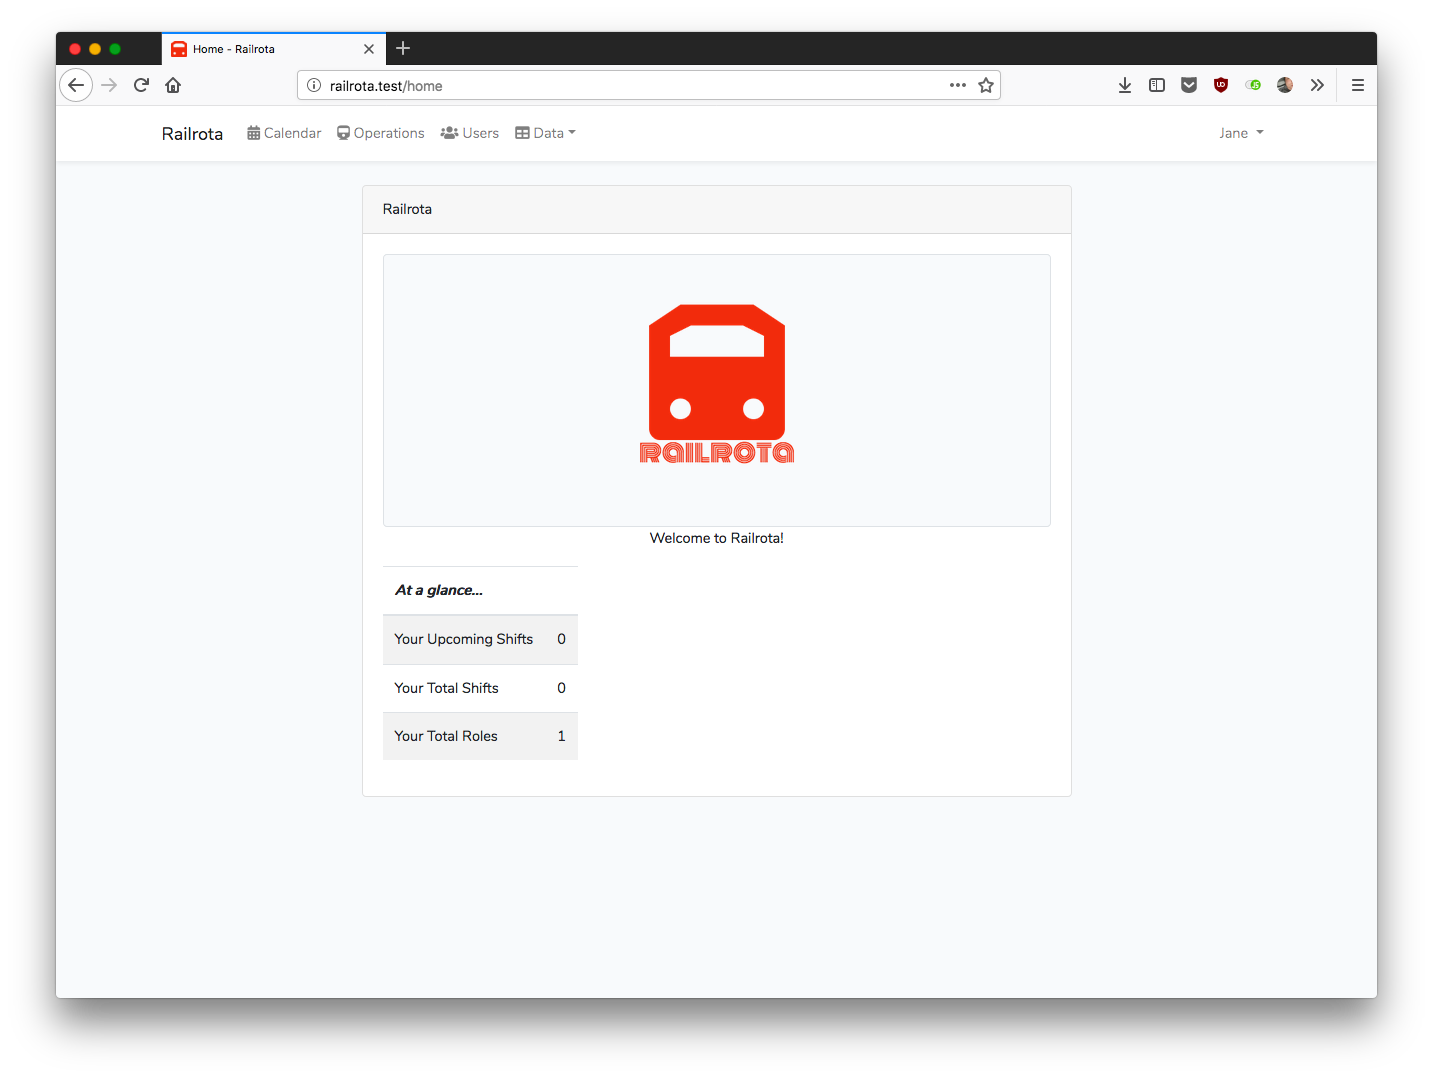
\includegraphics[width=1.0\textwidth]{Figures/screenshot-homepage}
    \caption{Screenshot of the homepage displayed after authentication.}
    \label{fig:homepage-screenshot}
\end{figure}

The homepage view, which behaves as the application's actual homepage when the user has logged in, shows some convenient information on that volunteer's upcoming shifts, and their total number of shifts so far. This is different to the much more simple 'welcome' view, that is displayed to an unauthenticated user when they first navigate to the application's web address, and prompts the user to login.

\begin{figure}[!ht]
    \centering
    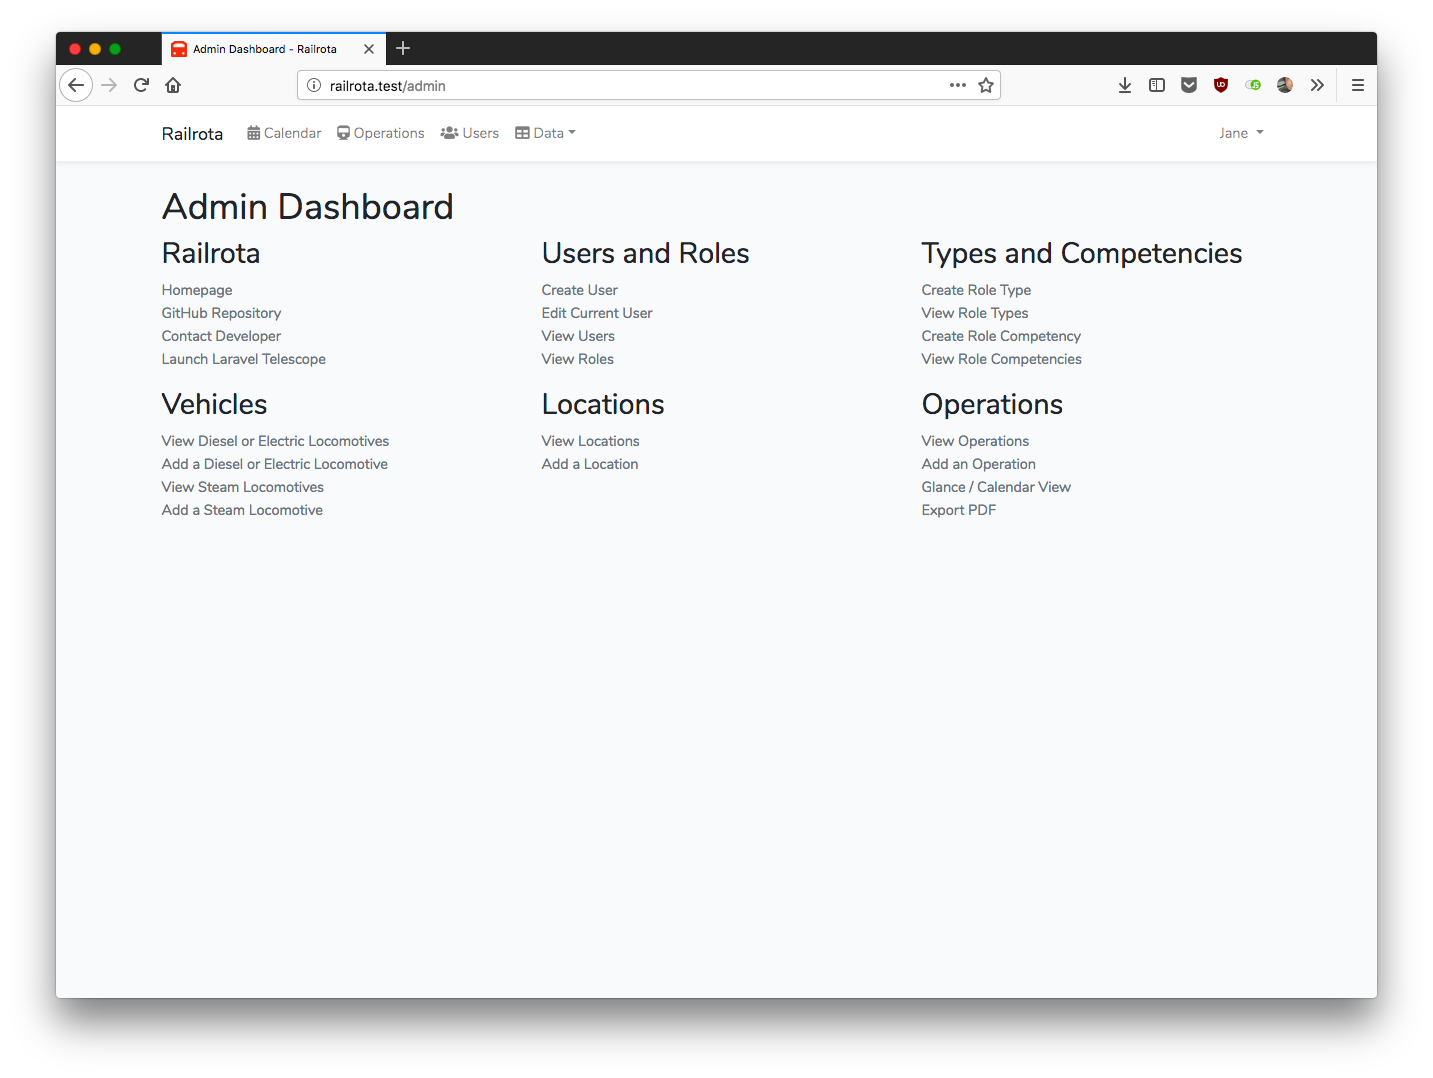
\includegraphics[width=1.0\textwidth]{Figures/screenshot-admin}
    \caption{Screenshot of the administration panel, only accessible by users with administrative rights.}
    \label{fig:adminpanel}
\end{figure}

Administrators also have access to an administrative panel - though this view does not provide any additional functionalities by itself per se, it does provide quick links to resources pages that an administrator might need to access when adding or changing elements of the application. It also provides a convenient link to the diagnostic tool Laravel Telescope, explored in further detail in Chapter 6.
\chapter{Testing}

\section{Introduction}

Software testing is an integral part of agile software development - with the use of Feature-Driven Development, it is important to know when a feature has reached the state of 'done', and this is typically once automated tests have confirmed that the functionality works as intended. \cite{Karam1} Radigan explains that incorporating agile testing practices, such as those used in FDD or Test-Driven Development (TDD) are a great way of minimising technical debt, and allowing for QA (Quality Assurance) staff to 'keep up with development'. \cite{Radigan1}

The Laravel framework is reportedly built for 'testing in mind', and PHPUnit, a xUnit (akin to JUnit) testing framework for PHP developed by Sebastian Bergmann is included by default. There are also browser-facing testing tools included under Laravel Dusk, but due to time-constraints were omitted. The automated tests used by this application were therefore all written in PHPUnit. \cite{Laravel10} \cite{Bergmann1}


\section{Automated Testing}

\begin{figure}[!ht]
    \centering
    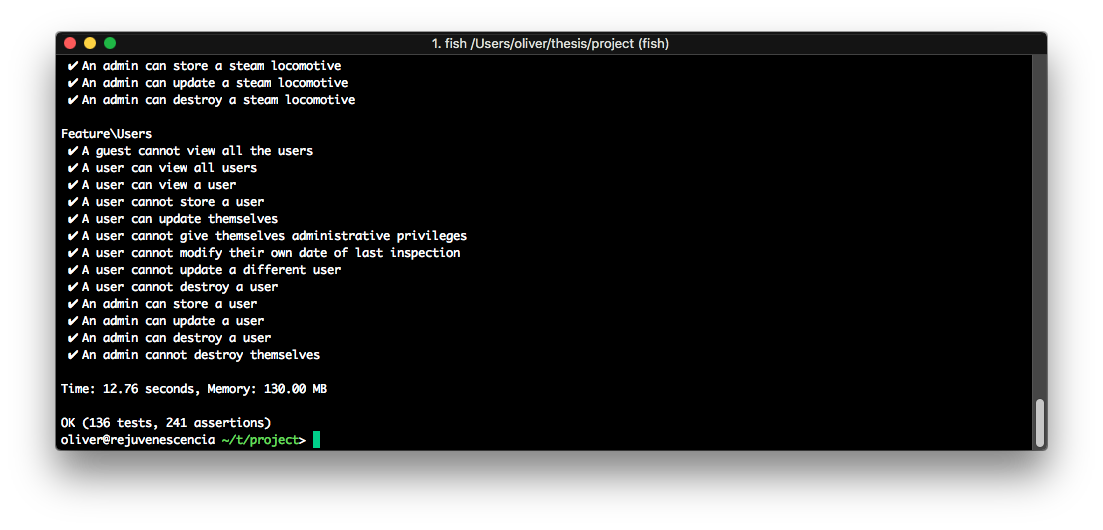
\includegraphics[width=1.0\textwidth]{Figures/tests}
    \caption{Screenshot of PHPUnit running, and successfully running all available tests.}
    \label{fig:testscmd}
\end{figure}

Two subdirectories are defined within the tests directory, one for unit tests, and the other for feature testing. All tests from both subdirectories are executed when PHPUnit is directed to begin testing. Two base classes also exist within this parent directory for subsequent tests to extend from; these files are provided by Laravel. \cite{Laravel10}

A characteristic shared by both types of test is their use of a \texttt{setUp} method, which can set up certain parameters for testing, such as the use of a predefined volunteer user or administrator user for testing, so that they do not need to be set up with each test. \texttt{DatabaseMigrations} is also imported into the class to instruct PHPUnit to ensure that database migrations are ran before testing commences, so that tests do not attempt to run on a blank dummy database, and subsequently fail as tables they depend upon, do not exist. \cite{Laravel10}

Finally, all tests are written with method names resembling sentences, with a prefix of 'test'. This is so that when tests are run, as shown in figure \ref{fig:testscmd}, the purpose of each test is parsed into a readable sentence.

\textbf{The full results of unit and feature testing can be found in Appendix \ref{Automated Test Results}.}

\subsection{Unit Testing}
Unit tests are designed to test very specific parts of the application, such as specific methods within classes. According to Hamill, a unit test should 'test a particular behaviour within the production code. Its success or failure validates a single unit of code'. \cite{Hamill1}

An example unit test is this code taken from one of the program's unit test classes:

\begin{lstlisting}[language=PHP, breaklines]
    public function test_an_operation_shift_can_derive_its_parent_operation()
    {
        $this->assertNotNull($this->getShift()->create()->operation);
    }
\end{lstlisting}

The purpose of this test can very quickly be derived from its method name - that it checks whether a shift can derive its parent operation. As nested resources, all shifts must be attached to some resource, and if the associated operation cannot be derived using an Eloquent method (i.e. \texttt{\$shift->operation}) then that shift is likely to be orphaned, or a regression has happened somewhere that has broken the relationship defined between the classes. Unit tests exist to ensure that these regressions are picked up on as immediately as they occur, a concept known as regression testing. \cite{Hopping1}

\subsection{Feature Testing}
In contrast to unit tests, feature tests test complex behaviour that can span across different methods. The approach here is that for each resource, every route is tested for the appropriate response in accordance with expected behaviour, combined with the use of negative testing - to ensure that behaviour that a user should not be able to is accounted for as best as possible. \cite{Fornal1}

\begin{lstlisting}[language=PHP, breaklines]
    public function test_an_admin_can_store_an_operation()
    {
        $this->actingAs($this->admin);
        $operation = factory('App\Operation')->make();

        $response = $this->post(route('operations.store'), $operation->toArray());

        $response->assertRedirect();
        $this->assertDatabaseHas('operations', [
            'is_running' => $operation->is_running,
            'notes' => $operation->notes,
        ]);
    }
\end{lstlisting}

In this test, the entire \textit{operation.store} route is tested to ensure that those with administrative privileges can create new operations. An administrator has already been built by the testing suite, so the \texttt{actingAs} method tells PHPUnit that user will be used to carry out actions and will be authenticated as such. An operation is then generated, and the test attempts to POST this to the route, as would normally happen by a HTML form. The response to this is stored within \texttt{\$response} for assertions to be made against its contents.

PHPUnit is expecting the response to have redirected the user, and then proceeds to check that the database contains the operation that was posted. If this is the case, then we know that this was successful.

The reverse test equivalent to this checks that users cannot attempt to store operations of their own, like thus:

\begin{lstlisting}[language=PHP, breaklines]
    public function test_a_user_cannot_store_an_operation()
    {
        $this->actingAs($this->user);
        $operation = factory('App\Operation')->make();

        $response = $this->post(route('operations.store'), $operation->toArray());

        $response->assertForbidden();
        $this->assertDatabaseMissing('operations', [
            'is_running' => $operation->is_running,
            'description' => $operation->description,
        ]);
    }
\end{lstlisting}

The test works in a near identical way, with the same preliminary actions being taken, except this time a pre-generated user without admin privileges has been used. The assertions however this time, are that instead of being redirected, that the application has returned a HTTP 403 Forbidden error code, and that the entry created has not been saved to the database.

\section{Manual Testing}
Some manual testing was done to complement the automated test coverage, primarily for the authentication routes - being able to log in, log out, register, and reset a password. Though automated testing is used for the vast majority of the application behaviour, manual testing can be complementary for behaviour that is user-focused and not 'black-and-white' - Nordeen goes on to explain the importance of both in parallel: 'testers must dispel old black-and-white notions of manual testing versus automation testing. Both have their place in modern software development, and it's more a matter of knowing when and where to use each.' \cite{Nordeen1}

Manual testing tables are available on Appendix \ref{Manual Test Results}.

\section{Laravel Telescope}

\begin{figure}[!ht]
    \centering
    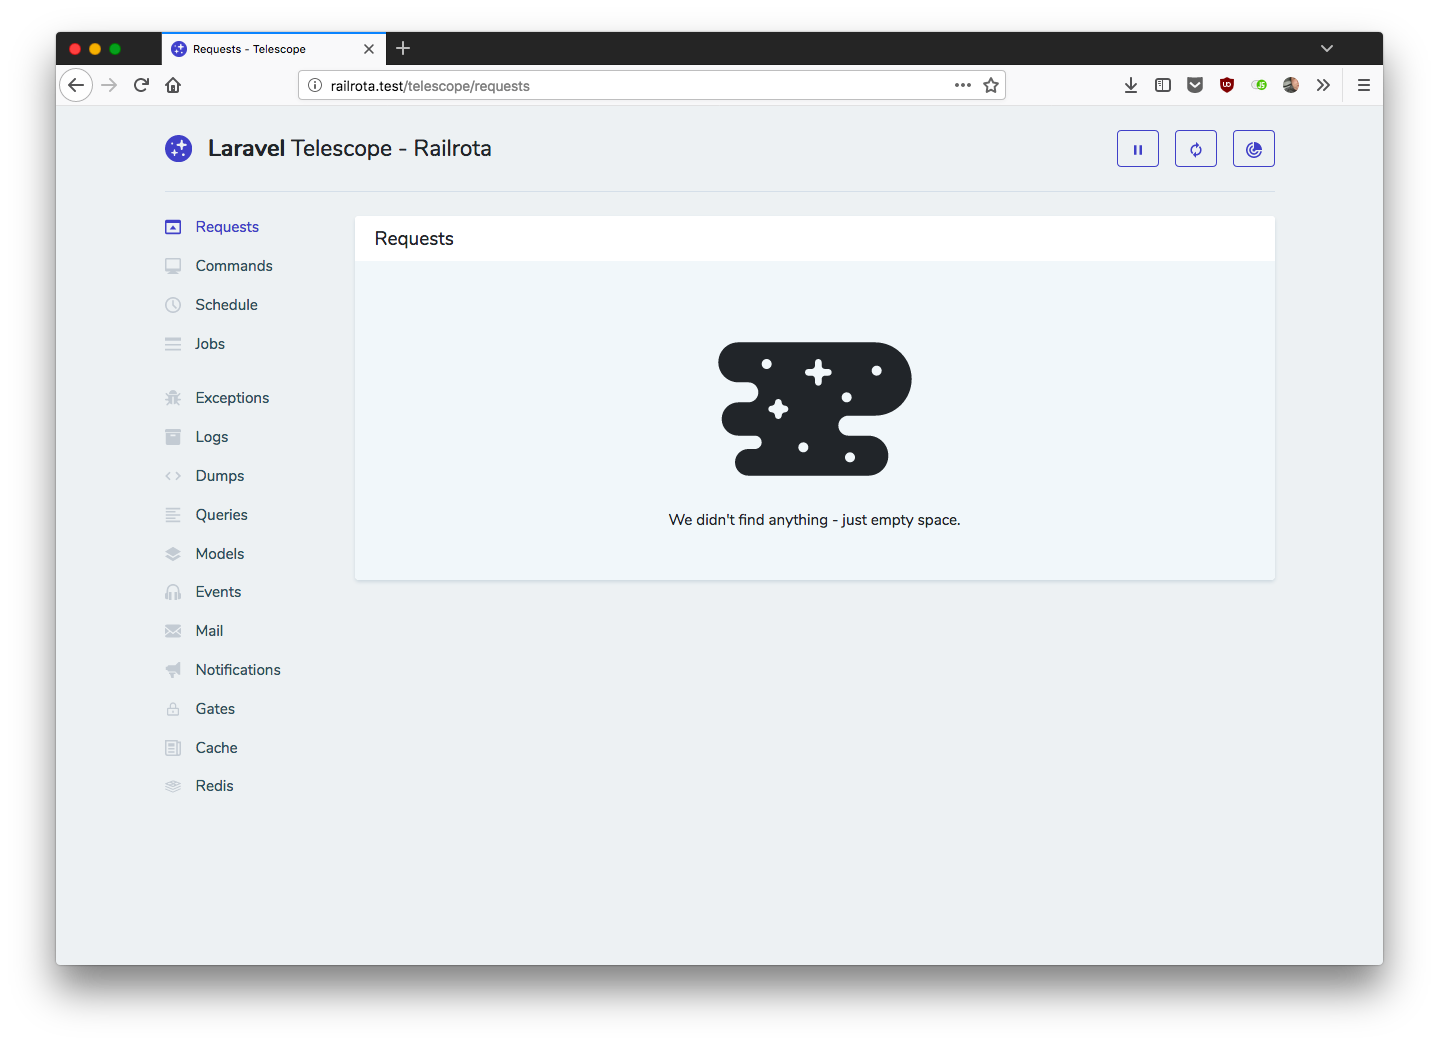
\includegraphics[width=1.0\textwidth]{Figures/screenshot-telescope}
    \caption{Screenshot of the Laravel Telescope interface.}
    \label{fig:telescope}
\end{figure}

Telescope is a debug assistant, that allows authorised users to inspect recent database queries, recent exceptions, log entries, and other useful information for diagnosing problems with the application. This is incredibly useful in the development process, but can be helpful for quickly uncovering problems in production also. \cite{Laravel11} \cite{Abati1}

It is not automatically included or installed with Laravel and must be installed manually. Admin users that are authorised to access Telescope whilst it is running in production mode can be defined by their IDs within the \texttt{.env} environment file.

This functionality was left included as it was immensely useful during the development process to simplify the often tedious and complex process of debugging PHP, and as it is protected by authentication and authorisation, there are no immediate downsides leaving it in the codebase.
\chapter{Deployment}

\section{Composer}

\section{Laravel Mix}

\section{Deployment Process}

\subsection{Deployment Script}

\subsection{Manual Deployment}

\subsection{Generating Documentation}
\chapter{Critical Evaluation}

\section{Introduction}
The aims of this chapter are to provide a critical analysis and evaluation of various aspects of the development process, including providing insight into what could have been done better and the various shortcomings that could have been approached better throughout the life-cycle of the project. 

\section{Implementation of Requirements}

\subsection{Functional Requirements}
The requirements that were successfully implemented for this release of the project are as follows:

\begin{itemize}
    \item All users must be able to navigate the roster, and view current, upcoming, and/or historic shifts
    \item Users must be able to fill in and edit their personal information
    \item Users must be able to assign themselves to shifts of which they are able to do
    \item Users must \textbf{not} be able to assign themselves to shifts that they are unable to do
    \item Users must be able to indicate periods of availability
    \item Users must be able to operate the web application easily from a mobile device such as a smartphone
    \item Administrators must be able to modify user information
    \item Administrators must be able to assign roles and privileges that reflect a volunteer's ability and status
    \item Administrators must be able to add, edit, and delete shifts
    \item Administrators must be able to mark a shift as closed
    \item Administrators must be able to define a shift's staffing requirements
    \item The application must run on a predetermined operating environment
\end{itemize}

The behaviours that were not successfully implemented are:

\begin{itemize}
    \item Users must \textbf{not} be able to assign themselves to simultaneous roles on the same shifts
    \item Users must be able to indicate their willingness or desire to do an upcoming shift (i.e. an unspecified upcoming weekend)
    \item Administrators must be able to email users regarding upcoming shifts
\end{itemize}

The first of these two requirements was intentionally left out after a conversation with the client, where it was expressed that it was certainly possible for a particular volunteer to be carrying out more than one role, although unlikely, during an operation. This might be the case for example where an experienced member of staff is monitoring a trainee, whilst also carrying out some miscellaneous function. Nevertheless, should the customer change their mind on this and wish to have this requirement reinstated, it could be reverted in a straightforward manner.

The next point, being able to indicate willingness or desire to do an upcoming shift was actually overlooked and, due to human error, not implemented before development was frozen. While embarrassing, an important lesson can be learned from this experience on the importance on continuously ensuring and checking that requirements are being met at all stages of the project, and that any ongoing work should be directly attributable to a requirement, such as by using user stories. 

Lastly, the functionality to email users with upcoming shift information was simply not able to be implemented in time for the initial software release, purely a result of time constraints. This was communicated to the customer as a matter of urgency; reassuring them that it would be included in a future revision of software, and was met with approval.

Despite having missed three functional requirements within the first release, this success rate of 80\% is nevertheless a positive one, especially given that changes and feedback were continuously exchanged throughout the development process. This should be considered a successful delivery of functionality, which ultimately is the key indicator of progress and success in an agile software project. \cite{beck2001agile}

\subsection{Desirable Functionality}

Automated rostering was considered beyond the scope of this release due to it being a complicated computational problem, and following discussion with the customer, it was deemed not to be an issue, but perhaps functionality that could be considered in a distant future release as the number of railway volunteers increases. They also stressed that they did not want optional automated rostering from potentially complicating the UI of the application, which was what initially prompted its inception in the first place, as existing solution HOPS was considered too complex for the average user to navigate.

The ability to implement localisation into the program was researched and was considered for the first release. Ultimately however, time constraints made it necessary to triage this functionality for a future release. This was discussed with the customer, as due to the high number of Welsh speakers in Machynlleth \cite{Census1} this might be a greater priority than an initial analysis might reveal. The customer nevertheless provided reassurance that it was not necessary for a first release of the software, but would gladly welcome it in a future revision.

\section{Adherence to Agile Methodology}
Overall adherence to the hybrid FDD methodology was mostly successful, with the Build by Feature iteration taking up the vast majority of development time, and fitting comfortably within the predetermined time-frame. However, one of the major violations of this methodology that happened periodically was not producing unit or feature tests as components were developed, and simply moving onto the next feature or route - without a concrete indication of behaviour being done. In order to rectify this, substantial time had to be allocated to going back and ensuring adequate test coverage was in place to prevent any accidental regressions in behaviour.

Furthermore, it was difficult to remain within the confines of the time-frames used in place of Scrum sprints. With all the best planning and foresight in the world, certain real life events can occur that can be problematic obstacles for solo developers who do not have other software engineers whom they can delegate work to when problems arise. In spite of these difficulties, 80\% of planned required functionality has made it into the initial release, showing a great deal of adaptability and resourcefulness on the developer's behalf, which are crucial elements in agile software development in a world where, for better or for worse, programmers do not have psychic abilities.

\section{Difficulties Encountered with Domain Knowledge}
By far the greatest difficulty with this project was wrestling with an onslaught of specific domain knowledge and terminology unique to railways, steam railways, and the work carried out thereon. Whilst the customer made every effort possible to ensure a wealth of documentation and terminology guidelines were available, it remained nevertheless difficult to fully assimilate without slowing down development efforts. Some problems did arise from confusion regarding specific terminology at multiple points in development, but thankfully due to regular meetings with the client these problems were diagnosed early and could be quickly rectified with further clarification and insight from the customer. 

This truly demonstrates the importance of face-to-face meetings, or in this instance, oral conversation, where information can far more readily be transferred from customer to developer without the need of lengthy or confusing documentation. This theory is backed up by Chow et al who identified customer involvement as a strong indicator for success in agile projects. \cite{CHOW2008961}

In a nutshell, when faced with a project that requires a substantial deal of domain knowledge or expertise, it is best to communicate with those with that expertise, i.e. the customer, as much as possible so that any issues can be quickly rectified and that large portions of the codebase need not be re-engineered.

\section{Suitability of Development Choices}
The use of a framework like Laravel drastically reduced the amount of boilerplate code that would normally need to be written for an application. Not a single line of SQL (Structured Query Language) was even needed to be written for the program due to the amount of heavy lifting that the Eloquent ORM is capable of doing. For these reasons especially, the choice of Laravel for a development framework (and subsequently PHP as a language) was a fitting and appropriate choice. After speaking informally with a colleague who was embarking on a similar but unrelated endeavour using vanilla PHP, it became apparent just how much database code that they had to write, which could be replicated with a simple Eloquent method under Laravel.

It is believed however that the use of Python and Django together would have been equally as sufficient as the offerings of said framework are similar, but this would have involved significantly more learning, and with some of the real life obstacles that slowed down development, this could have caused further unnecessary delays. It can be concluded that choosing a fully featured framework was the correct choice, instead of potentially needing to 'reinvent the wheel' by either using a more cut down framework like Express, or using no framework at all. This is really evident when one evaluates how much code and checks must be put into place for a comprehensive and secure authentication and authorisation system to work, but with Laravel, one only needs to put into place policies and call the appropriate method. \cite{Laravel8}

\section{Improvements to Testing Methodology}
Whilst the automated and manual test coverage is great and covers almost all Railrota functionality, one crucially missing element from the testing is ensuring that the application is easy to use for the customer - as the customer, or any other prospective volunteer, has not had the opportunity to test-run the software, besides being shown video demos during meetings.

A major improvement to the testing methodology that should be rectified in the future, would be to host regular meetings with the customer, and preferably prospective users, and allow them to operate the software freely and without prompt - recording their behaviour and feedback to make improvements to the user experience. (UX)

\section{Shortcomings and Recommendations for Further Releases}
Whilst the software is generally good quality expected of a Master's level software engineer, it is not without flaws indicative of someone learning a web framework for the first time.

One of the most glaring code smells that would be come immediately obvious to any experienced developer is the re-usage of code, both within controllers and within Laravel Blade templates. Although effort has been undertaken to ensure that code is compartmentalised as much as possible so that it is not reused, particularly in controllers, there is a lot of code that simply gets repeated. Moving some of this shared code into shared methods, or simply redesigning the algorithms into more concise functions would help clean up a lot of this underlying programming.

Furthermore, while much of the web interface has been abstracted into partial templates for re-usage, there are large portions of Blade logic that are repeated, and more effort could be made to reduce their recurrence so that if something needs to be changed, it can be changed once, rather than in multiple positions. Due to time constraints during development, the decision of 'function over form' had to be undertaken, which is reportedly common in many agile projects. However, for future revisions, developers should look to undo these code smells and make the code more maintainable for future work.
\chapter{Conclusion}

A brief summary of all that has gone before.

May include some directions for future work.

%TC:ignore

\setemptyheader
\addcontentsline{toc}{chapter}{Appendices}
\chapter*{Appendices}
The appendices are for additional content that is useful to support the discussion in the report. It is material that is not necessarily needed in the body of the report, but its inclusion in the appendices makes it easy to access. 

For example, if you have developed a Design Specification document as part of a plan-driven approach for the project, then it would be appropriate to include that document as an appendix. In the body of your report you would highlight the most interesting aspects of the design, referring your reader to the full specification for further detail.

If you have taken an agile approach to developing the project, then you may be less likely to have developed a full requirements specification. Perhaps you use stories to keep track of the functionality and the 'future conversations'. It might not be relevant to include all of those in the body of your report. Instead, you might include those in an appendix. 

There is a balance to be struck between what is relevant to include in the body of your report and whether additional supporting evidence is appropriate in the appendices. Speak to your supervisor or the module coordinator if you have questions about this.

\pagebreak

% start the appendix - sets up different numbering
\fancypagestyle{plain}{%
%\fancyhf{} % clear all header and footer fields
\fancyhead[L]{\textsl{Appendix\ \thechapter}}
\fancyhead[R]{\textsl{\leftmark}}}

\appendix
\fancyhead[L]{\textsl{Appendix\ \thechapter}}
\fancyhead[R]{\textsl{\leftmark}}
\fancyhead[C]{}
\fancyfoot[C]{\thepage}
\renewcommand{\headrulewidth}{0.4pt}
\renewcommand{\chaptermark}[1]{\markboth{#1}{}}

\fancyhead[L]{\textsl{Appendix\ \thechapter}}
\fancyhead[R]{\textsl{\leftmark}}
\fancyfoot[C]{{\thepage} of \pageref{LastPage}}

% include any appendices here
\chapter{Third-Party Code and Libraries}

\textbf{Please note: } There are libraries and frameworks included with Laravel, such as Vue.js and Axios, but they are unused. Only libraries and frameworks listed here have been used in Railrota. They are however, compatible with Laravel's MIT licensing.

\section{Laravel Framework}
Laravel Framework - Laravel is the main PHP web framework that empowers the application. This includes features commonly used by the Railrota application, such as the Eloquent ORM for working with the database, the Carbon datetime library, the Laravel Blade templating engine, the Artisan command line tool, and Laravel Mix for compiling front-end assets. The framework is released using the MIT license. This framework was used without modification. 

https://github.com/laravel/laravel

\section{Laravel Telescope}
Laravel Telescope is an optional library for Laravel to aid with debugging. The library is released using the MIT license. This library was used without modification.

https://github.com/laravel/telescope

\section{dompdf-laravel}
DOMPDF Wrapper for Laravel - HTML/CSS rendering engine used for converting webpages into PDF pages. Laravel wrapper for the DOMPDF library. The library is released using the MIT license. This library was used without modification.

https://github.com/barryvdh/laravel-dompdf

\section{Sami}
Sami API Documentation Generator - A standalone tool used for compiling PHPDoc / docblock comments into full documentation in HTML form. The tool is released using the MIT license. This tool was used without modification.

https://github.com/FriendsOfPHP/Sami

\section{PHPUnit}
PHPUnit - unit testing suite included with Laravel, but as it is used in development and not in production, included as a separate entry here. The framework is released under the BSD-3 license. This framework was used without modification.

https://github.com/sebastianbergmann/phpunit

\section{Bootstrap 4}
Bootstrap - HTML/CSS and JavaScript framework for responsive web design. This framework was released under the MIT license. This framework was used without modification.

https://github.com/twbs/bootstrap

\section{jQuery}

jQuery - JavaScript library for DOM manipulation and used by Bootstrap. This library was released under the MIT license. This framework was used without modification.

https://github.com/jquery/jquery 

\section{Font Awesome}

Font Awesome - CSS framework used for inserting icons into front-end UIs. This framework's code is licensed under the MIT license, with the icons being released under the CC BY 4.0 License. This framework is used without modification. More information can be found under the framework's LICENSE file.

https://github.com/FortAwesome/Font-Awesome
\chapter{Ethics Submission}

This appendix includes a copy of the ethics submission for the project. After you have completed your Ethics submission, you will receive a PDF with a summary of the comments. That document should be embedded in this report, either as images, an embedded PDF or as copied text. The content should also include the Ethics Application Number that you receive. 
\chapter{Code Examples}

For some projects, it might be relevant to include some code extracts in an appendix. You are not expected to put all of your code here - the correct place for all of your code is in the technical submission that is made in addition to the Final Report. However, if there are some notable aspects of the code that you discuss, including that in an appendix might be useful to make it easier for your readers to access. 

As a general guide, if you are discussing short extracts of code then you are advised to include such code in the body of the report. If there is a longer extract that is relevant, then you might include it as shown in the following section. 

Only include code in the appendix if that code is discussed and referred to in the body of the report. 

\section{Random Number Generator}

The Bayes Durham Shuffle ensures that the psuedo random numbers used in the simulation are further shuffled, ensuring minimal correlation between subsequent random outputs \cite{NumericalRecipes}.

\begin{verbatim}
 #define IM1 2147483563
 #define IM2 2147483399
 #define AM (1.0/IM1)
 #define IMM1 (IM1-1)
 #define IA1 40014
 #define IA2 40692 
 #define IQ1 53668
 #define IQ2 52774
 #define IR1 12211
 #define IR2 3791
 #define NTAB 32
 #define NDIV (1+IMM1/NTAB)
 #define EPS 1.2e-7
 #define RNMX (1.0 - EPS)
 
 double ran2(long *idum)
 {
   /*---------------------------------------------------*/
   /* Minimum Standard Random Number Generator          */
   /* Taken from Numerical recipies in C                */
   /* Based on Park and Miller with Bays Durham Shuffle */
   /* Coupled Schrage methods for extra periodicity     */
   /* Always call with negative number to initialise    */
   /*---------------------------------------------------*/	
 
   int j;
   long k;
   static long idum2=123456789;
   static long iy=0;
   static long iv[NTAB];
   double temp;
 
   if (*idum <=0)
   {
     if (-(*idum) < 1)
     {
       *idum = 1;
     }else
     {
       *idum = -(*idum);
     }
     idum2=(*idum);
     for (j=NTAB+7;j>=0;j--)
     {
       k = (*idum)/IQ1;
       *idum = IA1 *(*idum-k*IQ1) - IR1*k;
       if (*idum < 0)
       {
         *idum += IM1;
       }
       if (j < NTAB)
       {
         iv[j] = *idum;
       }
     }
     iy = iv[0];	
   }
   k = (*idum)/IQ1;
   *idum = IA1*(*idum-k*IQ1) - IR1*k;
   if (*idum < 0)
   {
     *idum += IM1;
   }
   k = (idum2)/IQ2;
   idum2 = IA2*(idum2-k*IQ2) - IR2*k;
   if (idum2 < 0)
   {
     idum2 += IM2;
   }
   j = iy/NDIV;
   iy=iv[j] - idum2;
   iv[j] = *idum;
   if (iy < 1)
   {
     iy += IMM1;
   }
   if ((temp=AM*iy) > RNMX)
   {
     return RNMX;
   }else
   {
     return temp;	
   }
 }
 
\end{verbatim}


\chapter{Gantt Chart}
\label{Gantt Chart}

The Gantt chart that was used throughout the project to define the various stages of development, specify start and end dates for each phase, and to help provide context on the time-frame of the undertaking.

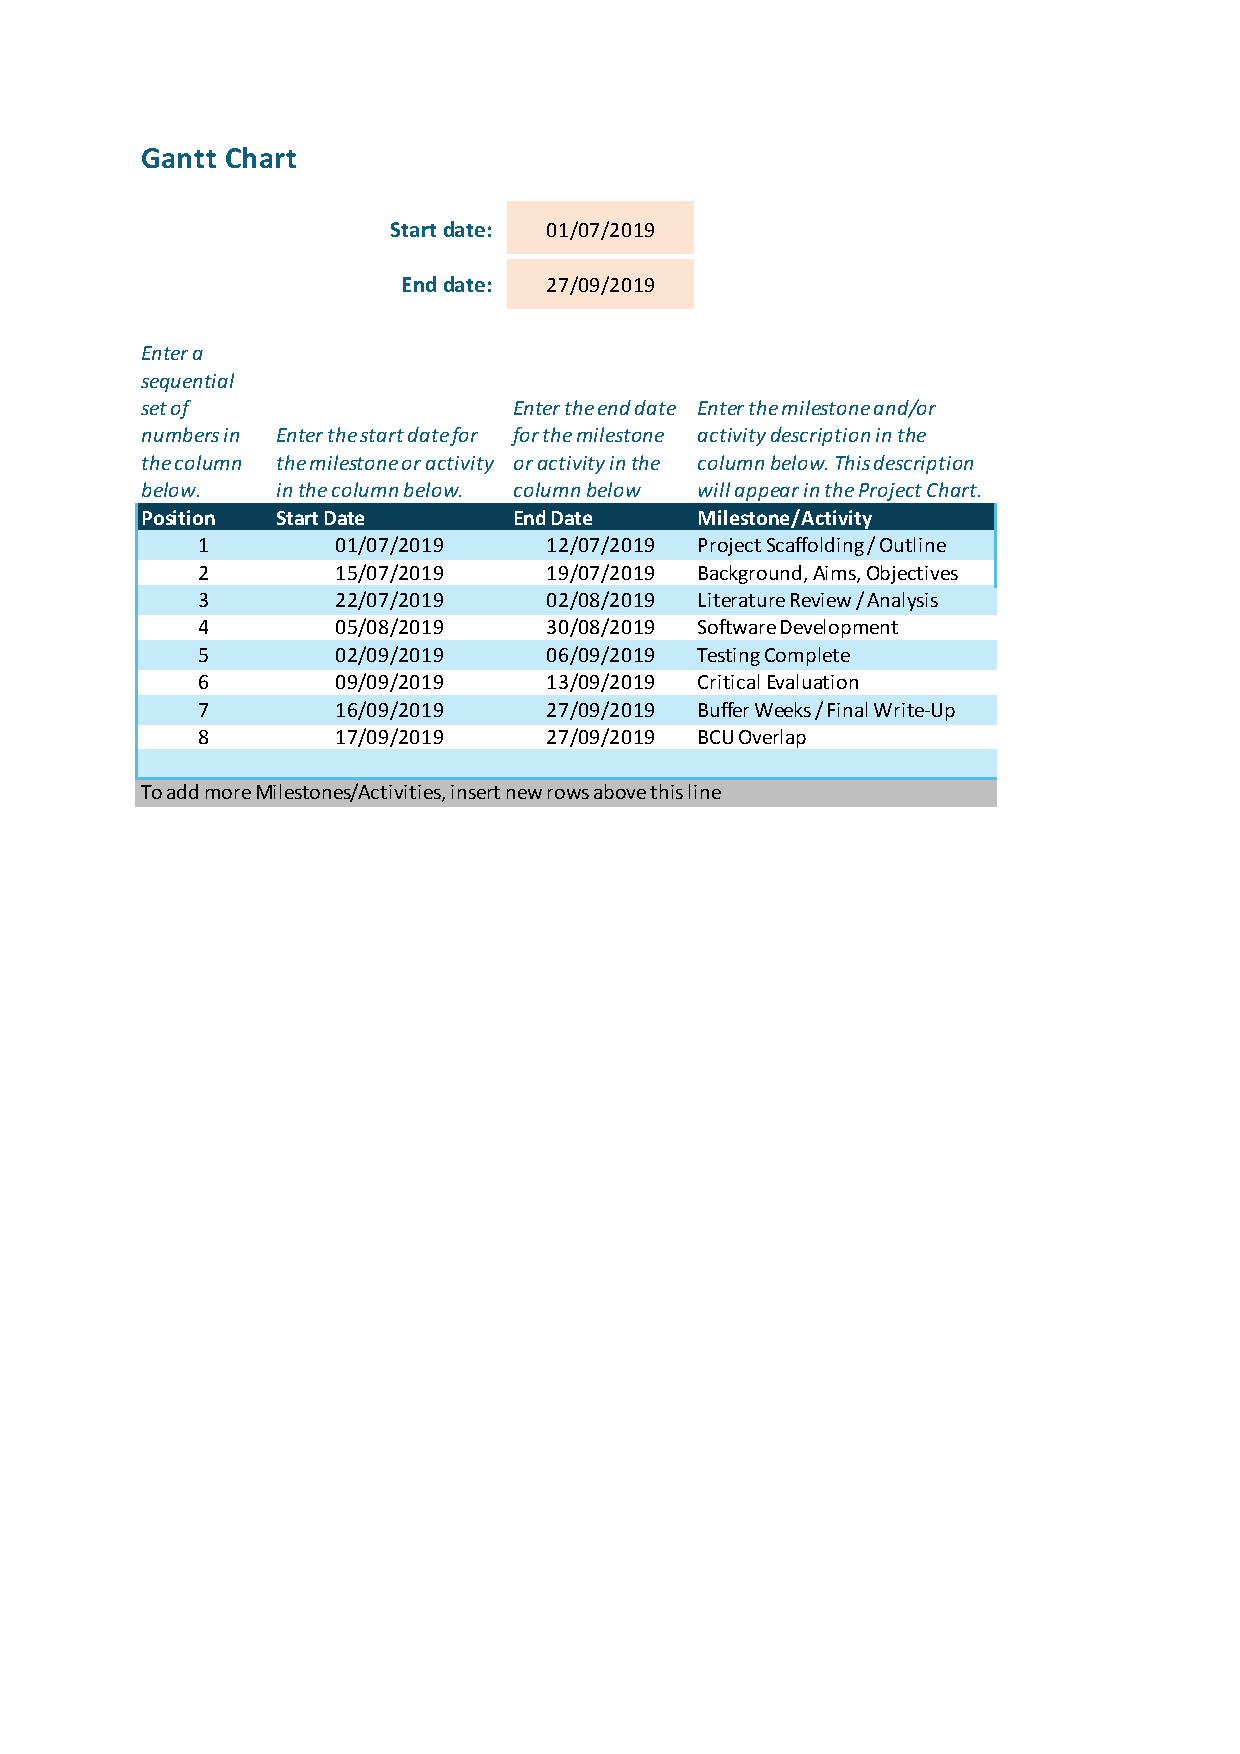
\includepdf[pages=-, pagecommand={}]{Appendix4/Gantt.pdf}
\chapter{Operating Environment}
\label{Operating Environment}

The following information was obtained in relation to the operating environment - a server located in the city of Amsterdam, Netherlands.

\begin{lstlisting}[breaklines]
rcs@silo:~$ cat /proc/cpuinfo 
processor    : 0
vendor_id    : GenuineIntel
cpu family    : 6
model        : 77
model name    : Intel(R) Atom(TM) CPU  C2350  @ 1.74GHz
stepping    : 8
microcode    : 0x127
cpu MHz        : 1745.626
cache size    : 1024 KB
physical id    : 0
siblings    : 2
core id        : 0
cpu cores    : 2
apicid        : 0
initial apicid    : 0
fpu        : yes
fpu_exception    : yes
cpuid level    : 11
wp        : yes
flags        : fpu vme de pse tsc msr pae mce cx8 apic sep mtrr pge mca cmov pat pse36 clflush dts acpi mmx fxsr sse sse2 ss ht tm pbe syscall nx rdtscp lm constant_tsc arch_perfmon pebs bts rep_good nopl xtopology nonstop_tsc aperfmperf pni pclmulqdq dtes64 monitor ds_cpl vmx est tm2 ssse3 cx16 xtpr pdcm sse4_1 sse4_2 movbe popcnt tsc_deadline_timer aes rdrand lahf_lm 3dnowprefetch ida arat epb dtherm tpr_shadow vnmi flexpriority ept vpid tsc_adjust smep erms
bogomips    : 3491.25
clflush size    : 64
cache_alignment    : 64
address sizes    : 36 bits physical, 48 bits virtual
power management:

processor    : 1
vendor_id    : GenuineIntel
cpu family    : 6
model        : 77
model name    : Intel(R) Atom(TM) CPU  C2350  @ 1.74GHz
stepping    : 8
microcode    : 0x127
cpu MHz        : 1745.626
cache size    : 1024 KB
physical id    : 0
siblings    : 2
core id        : 1
cpu cores    : 2
apicid        : 2
initial apicid    : 2
fpu        : yes
fpu_exception    : yes
cpuid level    : 11
wp        : yes
flags        : fpu vme de pse tsc msr pae mce cx8 apic sep mtrr pge mca cmov pat pse36 clflush dts acpi mmx fxsr sse sse2 ss ht tm pbe syscall nx rdtscp lm constant_tsc arch_perfmon pebs bts rep_good nopl xtopology nonstop_tsc aperfmperf pni pclmulqdq dtes64 monitor ds_cpl vmx est tm2 ssse3 cx16 xtpr pdcm sse4_1 sse4_2 movbe popcnt tsc_deadline_timer aes rdrand lahf_lm 3dnowprefetch ida arat epb dtherm tpr_shadow vnmi flexpriority ept vpid tsc_adjust smep erms
bogomips    : 3491.25
clflush size    : 64
cache_alignment    : 64
address sizes    : 36 bits physical, 48 bits virtual
power management:

rcs@silo:~$ cat /proc/meminfo 
MemTotal:        4022480 kB
MemFree:          146956 kB
MemAvailable:    2274316 kB
Buffers:          298592 kB
Cached:          1919940 kB
SwapCached:        19680 kB
Active:          2073608 kB
Inactive:        1386788 kB
Active(anon):    1027160 kB
Inactive(anon):   356332 kB
Active(file):    1046448 kB
Inactive(file):  1030456 kB
Unevictable:           0 kB
Mlocked:               0 kB
SwapTotal:       1074172 kB
SwapFree:         743280 kB
Dirty:                 0 kB
Writeback:             0 kB
AnonPages:       1225512 kB
Mapped:           111816 kB
Shmem:            141628 kB
Slab:             361412 kB
SReclaimable:     303860 kB
SUnreclaim:        57552 kB
KernelStack:        4368 kB
PageTables:        18012 kB
NFS_Unstable:          0 kB
Bounce:                0 kB
WritebackTmp:          0 kB
CommitLimit:     3085412 kB
Committed_AS:    3204708 kB
VmallocTotal:   34359738367 kB
VmallocUsed:      279104 kB
VmallocChunk:   34359401400 kB
HardwareCorrupted:     0 kB
AnonHugePages:         0 kB
HugePages_Total:       0
HugePages_Free:        0
HugePages_Rsvd:        0
HugePages_Surp:        0
Hugepagesize:       2048 kB
DirectMap4k:       91136 kB
DirectMap2M:     4065280 kB
\end{lstlisting}
\chapter{Concept Art}
\label{Concept Art}

The following are hand-drawn early artwork concepts before being expanded upon digitally, as part of the initial design and conceptualisation process.

% 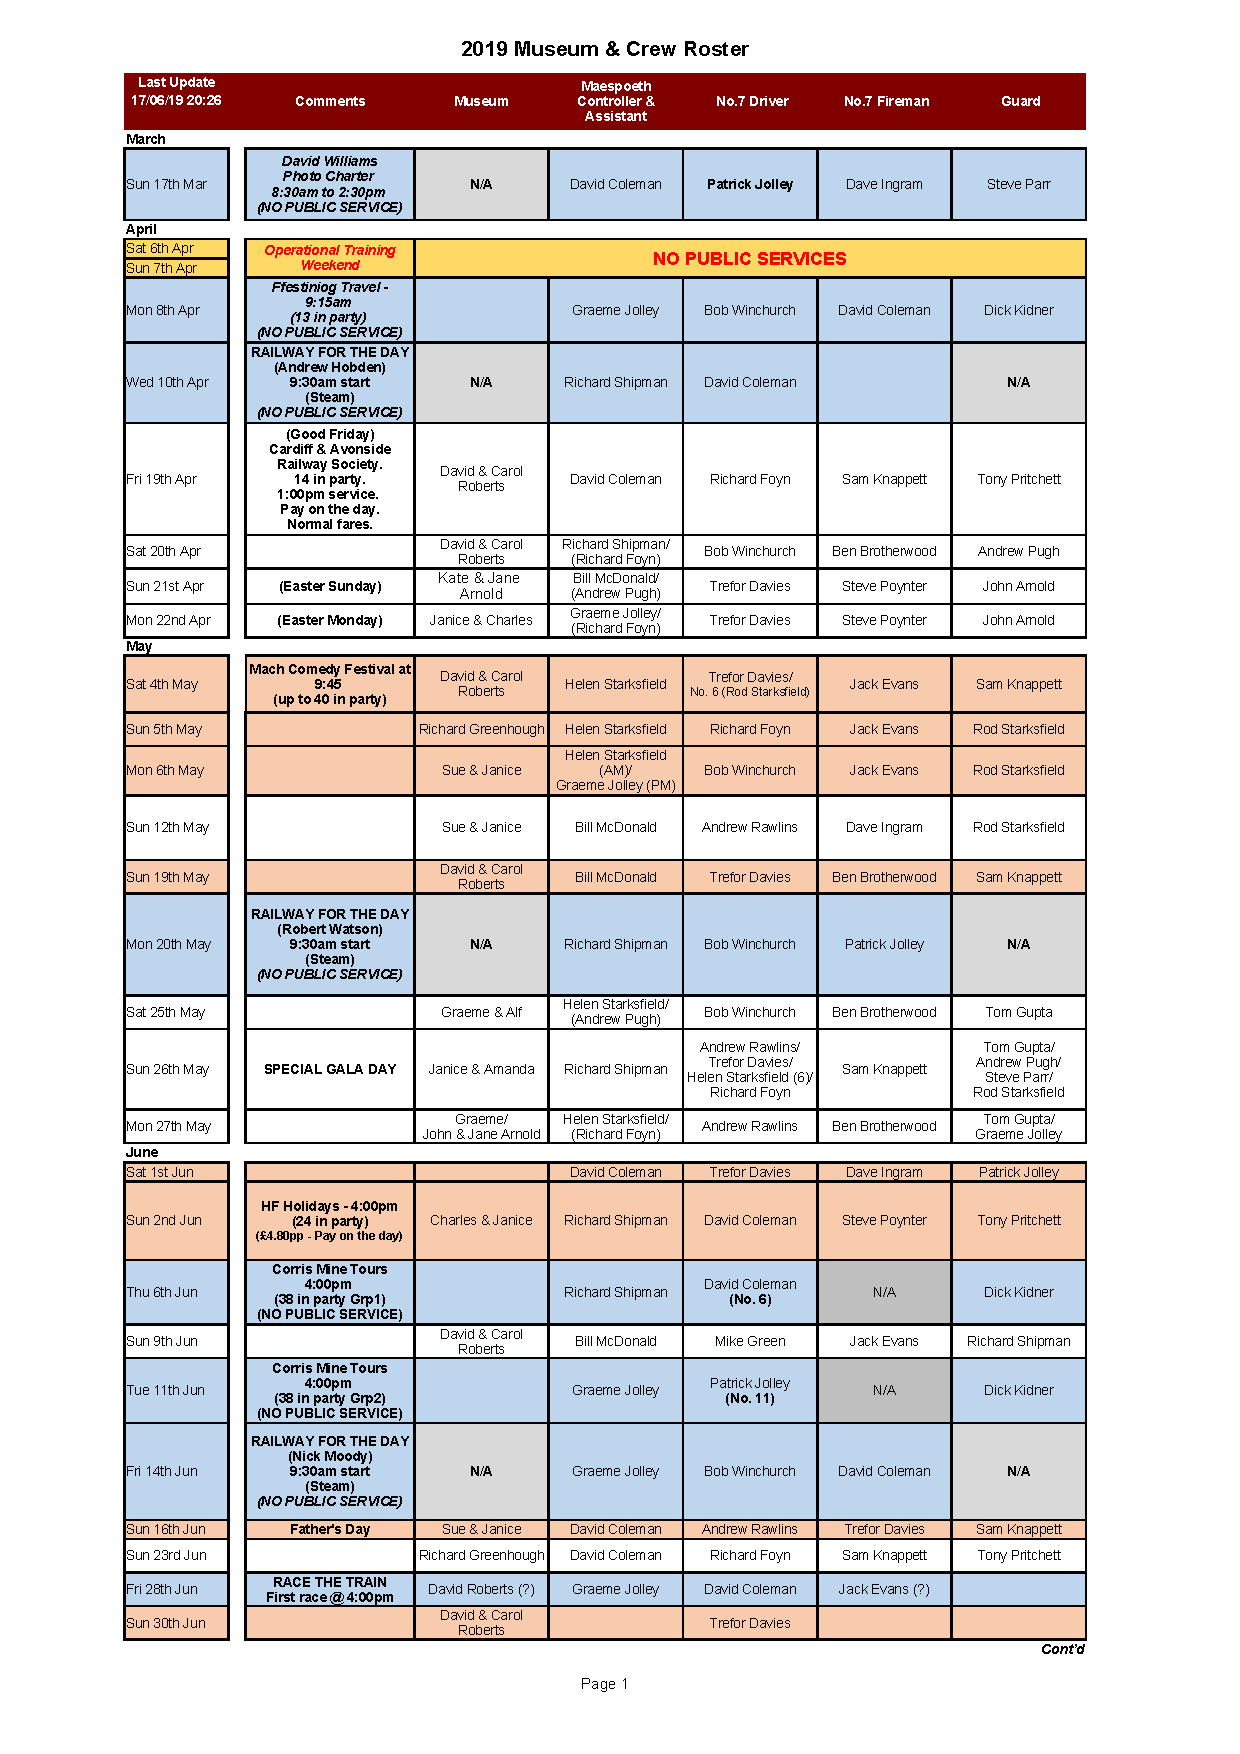
\includepdf[pages=-, pagecommand={}]{Appendix3/roster.pdf}
\chapter{Automated Test Results}
\label{Automated Test Results}

The following pages are HTML pages generated by PHPUnit.

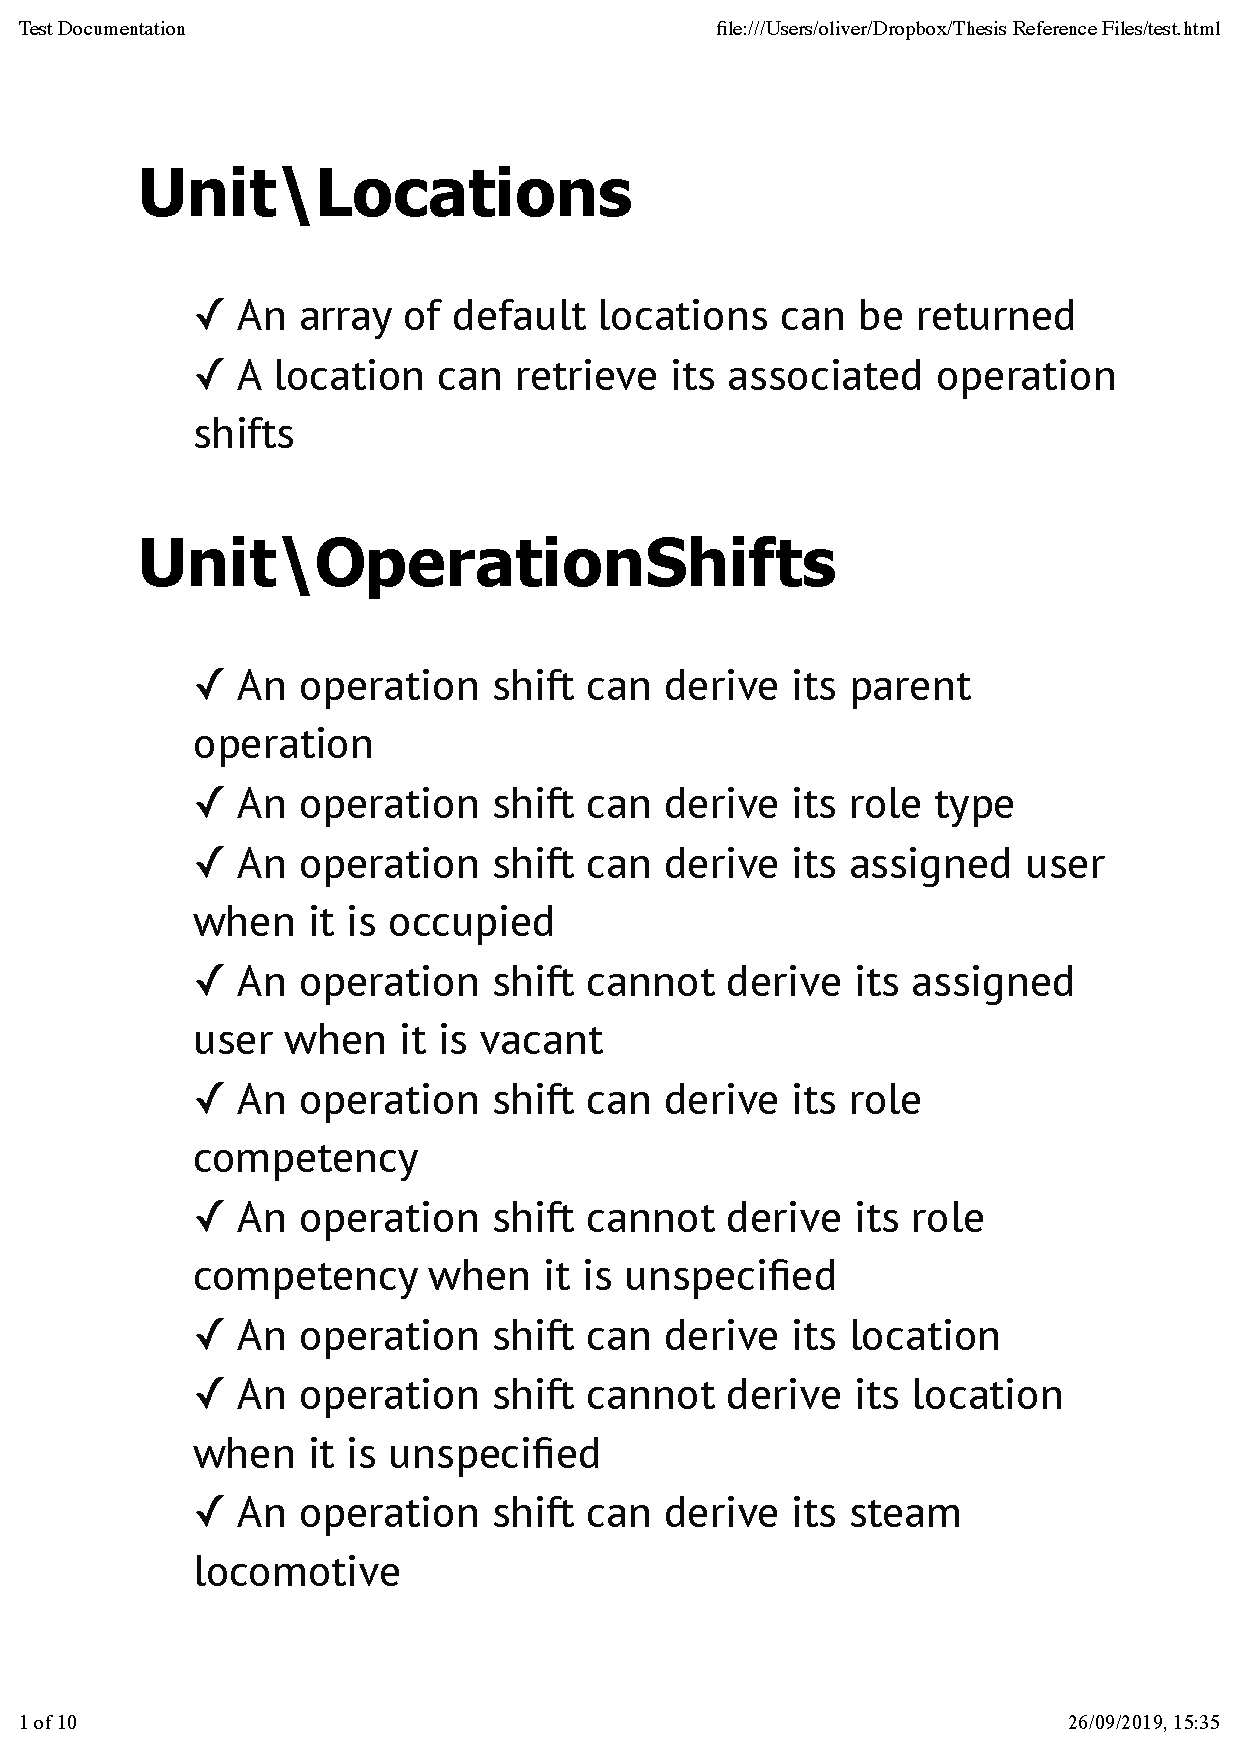
\includepdf[pages=-, pagecommand={}]{Appendix7/tests.pdf}
\chapter{Manual Test Results}
\label{Manual Test Results}

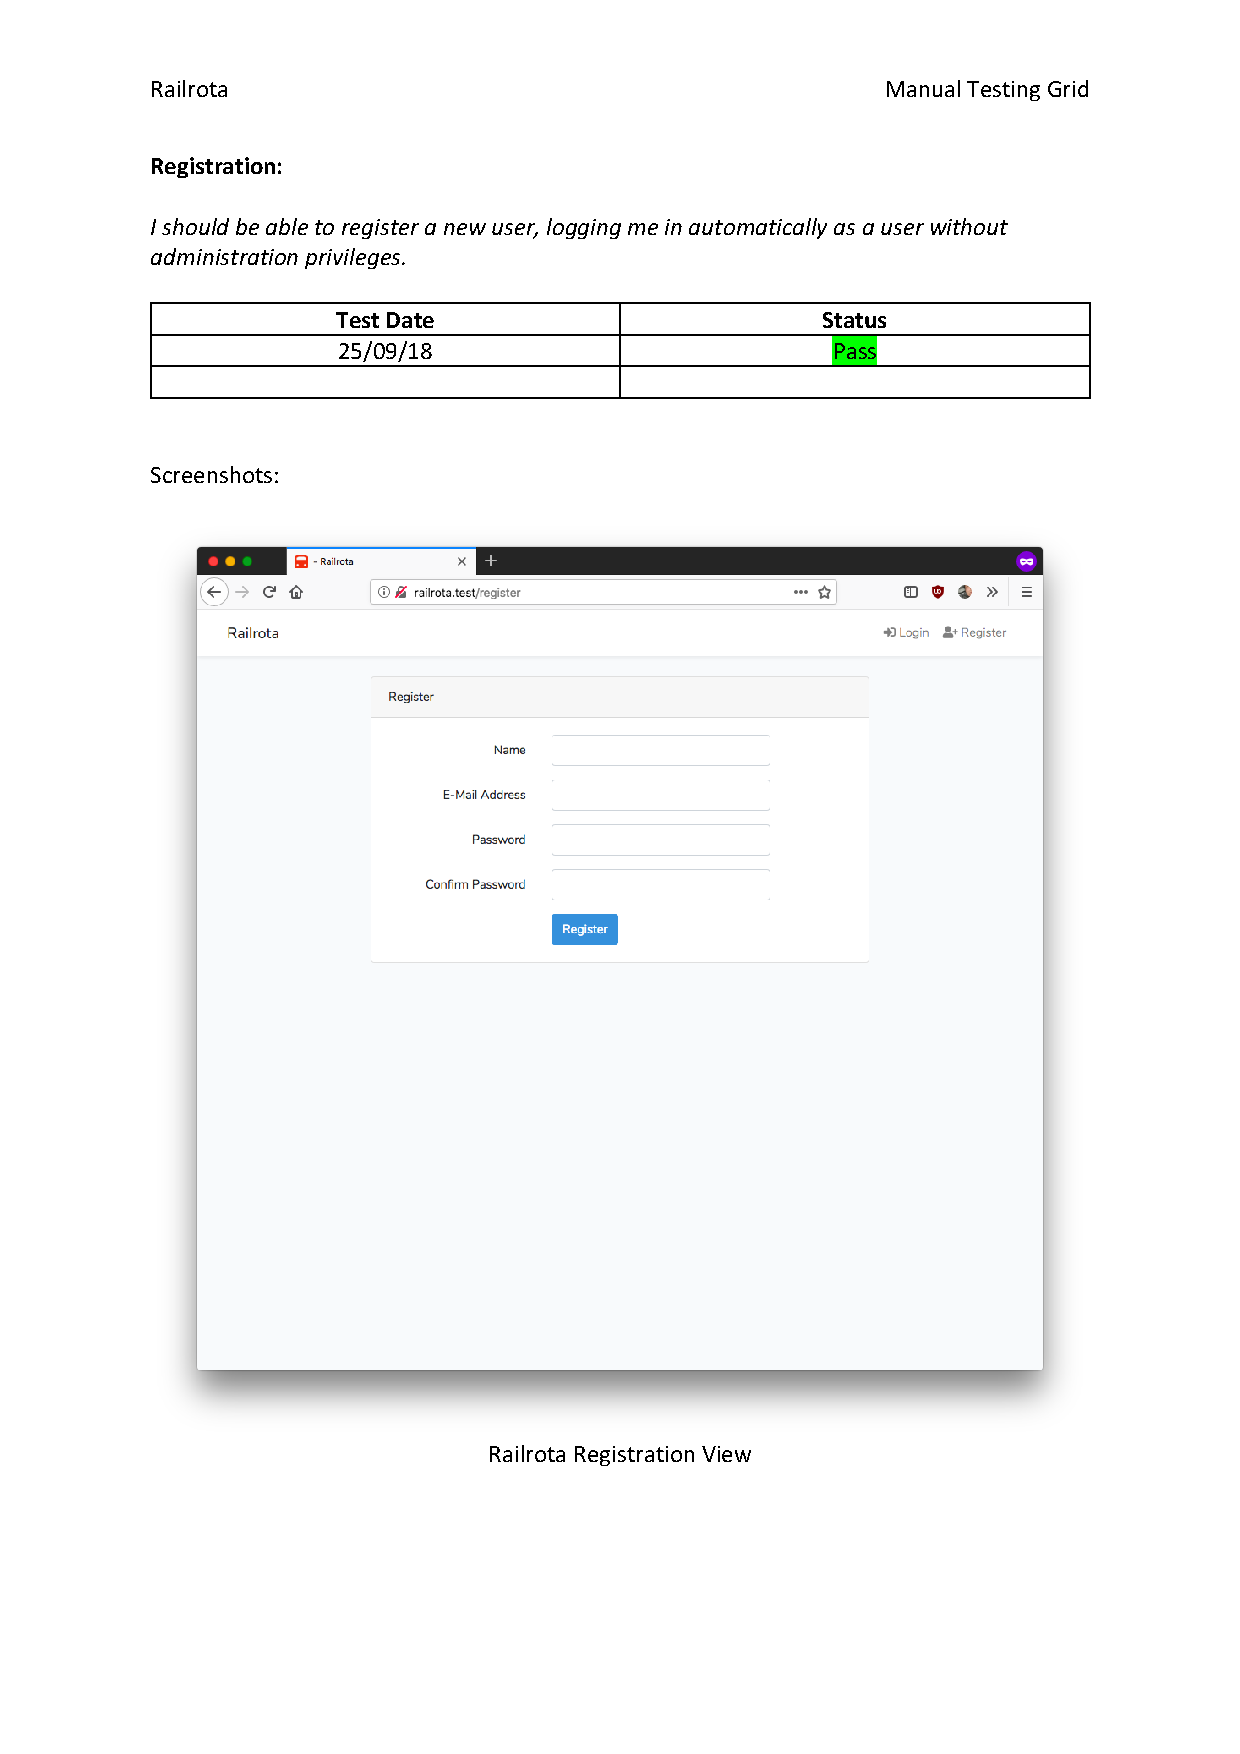
\includepdf[pages=-, pagecommand={}]{Tests/ManualTesting.pdf}

% Cheers for the fix Dan! (@dkmonaghan)
% https://github.com/digidol/MMP/pull/4
\fancyhead[L]{\textsl{}}
\fancypagestyle{plain}{%
   \fancyhead{} %[C]{Annotated Bibliography}
   \fancyfoot[C]{{\thepage} of \pageref{LastPage}} % except the center
   \renewcommand{\headrulewidth}{0pt}
   \renewcommand{\footrulewidth}{0pt}
}

\setemptyheader

\nocite{*} % include everything from the bibliography, irrespective of whether it has been referenced.

% the following line is included so that the bibliography is also shown in the table of contents. There is the possibility that this is added to the previous page for the bibliography. To address this, a newline is added so that it appears on the first page for the bibliography. 
\addcontentsline{toc}{chapter}{Annotated Bibliography} % Adds References to contents page

%
% example of including an annotated bibliography. The current style is an author date one. If you want to change, comment out the line and uncomment the subsequent line. You should also modify the packages included at the top (see the notes earlier in the file) and then trash your aux files and re-run. 
%\bibliographystyle{authordate2annot}
\bibliographystyle{IEEEannotU}
\renewcommand{\bibname}{Annotated Bibliography} 

\bibliography{References/references} % References file

%TC:endignore

\end{document}
